% ============================================================================
% RELATÓRIO FINAL DE INICIAÇÃO CIENTÍFICA DA UNIFEI (SIRDA)
% ============================================================================

\documentclass[12pt,a4paper]{article}

% --- Pacotes mínimos e amplamente disponíveis ---
\usepackage[utf8]{inputenc}
\usepackage[T1]{fontenc}
\usepackage[brazil]{babel}
\usepackage{mathptmx}
\usepackage{geometry}
\usepackage{xcolor}
\usepackage{graphicx}
\usepackage{booktabs}
\usepackage{setspace}
\usepackage{amsmath}
\usepackage{caption}
\usepackage{url}
\usepackage{titlesec}
\usepackage{indentfirst}
\usepackage{float}
\usepackage{tikz}
\usetikzlibrary{positioning, shapes.multipart, arrows.meta, calc, fit, backgrounds, shapes.geometric, shadows, shapes.symbols, shapes.misc}
% --- Página A4 e margens ---
\geometry{
  top=2.5cm,
  bottom=2.5cm,
  left=3.0cm,
  right=3.0cm
}

% --- Parágrafos e espaçamento geral ---
\setlength{\parindent}{1.25cm}
\setlength{\parskip}{0pt}
\setlength{\emergencystretch}{2em}
\onehalfspacing

% --- Legendas ---
\captionsetup{
  font=footnotesize,
  labelfont=bf,
  justification=centering,
  singlelinecheck=false
}

\newcommand{\fonte}[1]{\vspace{2pt} \begin{center} \footnotesize Fonte: #1 \end{center}}
\titleformat{\section}{\normalfont\fontsize{12}{15}\bfseries\uppercase}{\thesection}{1em}{}
\titlespacing*{\section}{0pt}{0.55cm}{0.3cm}

\begin{document}

% Inclusão do Cabeçalho e Resumo
% ============================================================================
% TÍTULO, AUTORES E IDENTIFICAÇÃO
% ============================================================================
\begin{singlespace}
\begin{center}
\textbf{AVALIAÇÃO DE DESEMPENHO DO APACHE DRUID: ESTRUTURAÇÃO DE EXPERIMENTOS E ANÁLISE COMPARATIVA}

\vspace{0.55cm}
Gabriel Gonçalves Sampaio\textsuperscript{1} (IC), Barbara Pimenta Caetano\textsuperscript{1} (PQ)

\vspace{0.15cm}
{\fontsize{9}{11}\selectfont\itshape
\textsuperscript{1}Instituto de Engenharia de Sistemas e Tecnologia da Informação (IESTI) - Universidade Federal de Itajubá (UNIFEI)\\
E-mails: gabriel@unifei.edu.br, barbara.caetano@unifei.edu.br}

\end{center}
\end{singlespace}

\vspace{0.3cm}

\begin{singlespace}
\begin{center}
\textbf{RESUMO}
\end{center}
O monitoramento geoespacial de desastres ambientais, especialmente o cruzamento em larga escala de incêndios florestais com infraestruturas críticas, exige arquiteturas de dados de baixa latência. Modelos tradicionais em lote (\textit{batch}) enfrentam gargalos severos ao correlacionar milhões de anomalias térmicas com fronteiras demográficas e elétricas do Brasil de forma interativa. Para avaliar uma alternativa escalável, este trabalho foca na estruturação de experimentos e na análise comparativa de desempenho do banco de dados analítico colunar Apache Druid, inserido em um fluxo \textit{DataOps} de processamento em tempo real. A metodologia envolveu a ingestão de 3,3 milhões de focos de calor históricos e sua correlação cruzada, na memória via \textit{Lookups}, com entidades como municípios, hospitais, malhas de transmissão elétrica e terras indígenas. A avaliação operacional baseou-se em testes de estresse progressivo (\textit{Query Per Second} - QPS) e no escalonamento horizontal de vCPUs e da segmentação do banco. Os resultados demonstram que estratégias compactas de alocação garantiram ganhos de vazão de até 38,8 vezes em relação a estratégias fragmentadas sob o mesmo hardware de 6 vCPUs. Adicionalmente, as avaliações de latência \textit{Percentil 95} (P95) indicaram que o sistema é capaz de resolver filtragens espaciais intensas em tempos que variam entre 2,8 a 8,2 segundos nos piores cenários de concorrência, suportando a carga sem estourar limites rígidos de RAM ($\sim$850 MB por nó na camada de cache). Conclui-se que o Apache Druid atende aos requisitos operacionais para inteligência geoespacial rápida, desde que a razão entre a taxa de requisições e a paralelização dos segmentos dos dados seja cuidadosamente calibrada.\\
\textbf{Palavras-chave:} Apache Druid. Benchmarking. DataOps. Processamento Analítico (OLAP). Monitoramento Geoespacial.

\vspace{\baselineskip}
\noindent\textbf{Área de Conhecimento:} Ciência da Computação\\
\textbf{Campus:} Itajubá
\end{singlespace}

\vspace{0.3cm}


\newpage
% Inclusão dos Capítulos
\section{Introdução}

As mudanças climáticas têm refletido na incidência de desastres ambientais no Brasil. Apenas no primeiro semestre de 2026, registraram-se 19.462 focos de incêndio \cite{poder360_2026}, complementando os registros de 2024, quando o fogo consumiu 30 milhões de hectares no país, predominantemente sobre florestas nativas na Amazônia \cite{g1_mapbiomas_2025}. A detecção isolada de anomalias térmicas satelitais, contudo, necessita ser correlacionada de forma contínua às vulnerabilidades demográficas e infraestruturais para subsidiar mitigações eficazes.

A integração de bases institucionais (INPE \cite{inpe_bdqueimadas_2026}, FUNAI \cite{funai_terras_2026}, ANEEL \cite{aneel_sigel_2026}, IBGE \cite{ibge_malha_2022}, DATASUS \cite{datasus_cnes_2026}) aos dados de satélite enfrenta profundos desafios de latência e padronização geométrica. Plataformas consolidadas, como o Painel do Fogo \cite{censipam_painel_2026}, prestam suporte essencial, porém arquiteturas de processamento baseadas em lotes (\textit{batch}) apresentam gargalos de vazão ao cruzar milhões de registros geoespaciais e séries temporais de forma interativa. Agregar massas de dados dinâmicas para a geração de respostas analíticas instantâneas permanece um limite técnico em sistemas tradicionais.

Diante dessa barreira, bancos de dados analíticos colunares (OLAP) orientados a \textit{streaming}, como o Apache Druid, despontam como soluções ideais para a absorção paralela de \textit{logs} em tempo real. Contudo, apesar de sua eficiência arquitetural no isolamento entre armazenamento e consulta \cite{yang_druid_2014}, ainda é incerto o impacto na latência quando tais motores são submetidos a volumétricas e complexas junções espaciais interativas (\textit{Lookups}) operando sob restrições severas de hardware e limitação de RAM.

Este trabalho tem como objetivo principal avaliar o desempenho e a estabilidade de processamento do Apache Druid frente a um rigoroso modelo de estresse analítico de dados geoespaciais e ambientais. Para ancorar o experimento em uma realidade aplicada, utiliza-se o SIRDA (Sistema de Inteligência e Resposta a Desastres Ambientais) como estudo de caso, implementando um fluxo \textit{DataOps} contínuo \cite{ereth_dataops_2018} capaz de consolidar riscos topológicos para a Defesa Civil.

O \textit{benchmark} estruturado revela que a otimização na compactação dos dados em segmentos possui um impacto superior ao aumento bruto de poder de processamento, registrando um ganho de 38,8 vezes na vazão de resposta frente a estratégias fragmentadas sob o mesmo hardware. Adicionalmente, os resultados destacam o fenômeno computacional \textit{Too Fast to Cache}, demonstrando que o sistema é capaz de resolver filtragens relacionais em tempos sub-segundo tão rapidamente que a contenção imposta à memória RAM pelo motor interno torna-se um limite arquitetural intransponível antes mesmo que as CPUs atinjam a saturação plena.

\section{Referencial Teórico}

Diante do gargalo tecnológico provocado pela fragmentação de bases de dados geográficas e ambientais, as agências de controle carecem de ferramentas capazes de prover uma visão unificada e contínua do risco sistêmico, um estado mental de percepção, compreensão e projeção frequentemente denominado pela literatura como Consciência Situacional \cite{endsley1995}. Desta forma, a principal vocação do SIRDA é fornecer inteligência acionável para órgãos de controle ambiental e de infraestrutura, tendo essa meta teoricamente embasada pelo modelo seminal de Mica R. Endsley.

Em seu trabalho \textit{``Toward a theory of situation awareness in dynamic systems''}, Endsley estipula que a Consciência Situacional não se resume à simples coleta de dados, mas divide-se obrigatoriamente em três grandes níveis cognitivos e sistêmicos: Percepção (Nível 1), Compreensão (Nível 2) e Projeção (Nível 3). Na arquitetura do SIRDA, a ingestão de anomalias térmicas via satélite (Nível 1) é cruzada geoespacialmente com infraestruturas críticas para determinar o contexto de risco (Nível 2), culminando em simulações topológicas que projetam o impacto iminente de incêndios sobre as redes de transmissão (Nível 3). É essa taxonomia que justifica plenamente o emprego de tecnologias de processamento de fluxos em tempo real (\textit{Streaming}) e de painéis interativos de resposta rápida que alimentam a camada analítica do projeto.

Para materializar essa estrutura complexa de Consciência Situacional sem ceder ao caos operacional de arquiteturas legadas, o SIRDA fundamenta-se nos princípios do DataOps. Diferentemente de abordagens tradicionais de rotinas ETL (Extração, Transformação e Carga), a plataforma assimila o DataOps conforme conceituado por Julian Ereth \cite{ereth_dataops_2018}. Em seu artigo \textit{``DataOps: towards a definition''}, Ereth formaliza que esse paradigma transcende a mera automação, caracterizando-se pela incorporação sistemática das práticas estruturadas da Engenharia de Software ao ciclo de vida da Engenharia de Dados. 

Para a gestão de catástrofes ambientais, essa abordagem teórica mostra-se indispensável. Quando o tempo de resposta é crítico, não há margem para erros estruturais nas tabelas ou quedas silenciosas de integração. A teoria de Ereth aplica-se ao nosso caso de uso por meio da imposição de tipagens estritas nos contratos de dados e na orquestração de alto nível dos processos. Isso evita que falhas em fontes primárias propaguem dados sujos ou geometrias inválidas para o banco de dados analítico final. A utilização de sistemas OLAP para a tomada de decisão é amplamente embasada na literatura \cite{chaudhuri_olap_1997}, sendo que a plataforma propõe a adoção deste conceito para o processamento de eventos escaláveis com o Apache Druid \cite{yang_druid_2014}. Tais práticas garantem que os gestores de crise tomem decisões pautadas em informações íntegras e validadas.

\section{Arquitetura e Especificações Técnicas}

A concepção do SIRDA (Sistema de Inteligência e Resposta a Desastres Ambientais) afasta-se do uso exclusivo de bancos de dados relacionais clássicos, adotando um ecossistema distribuído de \textit{Big Data} construído inteiramente sobre ferramentas de código aberto (\textit{open-source}). Esta escolha técnica provê escalabilidade ao acesso analítico e garante a capacidade de processar volumes massivos de anomalias térmicas, cruzando essas informações com geometrias complexas de infraestrutura em uma janela de tempo crítica. A arquitetura foi estruturada em torno das seguintes tecnologias:

\begin{itemize}
    \item \textbf{Apache Kafka:} Atua como o sistema nervoso central de mensageria, absorvendo picos severos de dados durante períodos críticos de queimadas, promovendo o desacoplamento entre a extração dos dados e a ingestão no banco analítico.
    \item \textbf{Apache Druid:} O motor OLAP (\textit{Online Analytical Processing}) escolhido pela sua capacidade nativa de ingerir fluxos de dados diretamente do Kafka (\textit{Streaming Ingestion}) e fornecer respostas analíticas em escala de baixa latência (poucos segundos).
    \item \textbf{PostgreSQL:} Empregado como o banco relacional de suporte, atuando estritamente como \textit{Metadata Store} para o Druid e para o sistema de visualização gráfica.
    \item \textbf{Dagster:} Orquestrador central que rege o paradigma DataOps do projeto. Ele garante a execução limpa, tipada e rastreável dos processos de enriquecimento espacial e publicação de mensagens no Kafka.
    \item \textbf{Apache Superset:} Camada visual que materializa o Nível 3 da Consciência Situacional, entregando painéis gerenciais e topológicos aos tomadores de decisão.
\end{itemize}

Para assegurar a reprodutibilidade e a portabilidade do sistema, a infraestrutura foi inteiramente conteinerizada via Docker. A topologia orquestrada no \textit{docker-compose} reflete fielmente um ambiente de produção resiliente. Destaca-se que o banco de dados analítico Apache Druid não foi instanciado como um serviço monolítico, mas sim desmembrado em seus microsserviços fundamentais: \textit{Coordinator}, \textit{Broker}, \textit{Historical}, \textit{MiddleManager} e \textit{Router}. Essa granularidade permite que a gestão de metadados, o roteamento de consultas e o processamento de dados ocorram em instâncias independentes, mitigando gargalos e falhas em cascata.

Além da separação lógica, a implantação local adota restrições físicas de hardware para mimetizar limitações produtivas reais. Foram aplicados limites explícitos de uso de processamento e memória RAM para cada serviço (\textit{deploy resources limits}) na configuração dos contêineres. Paralelamente, os parâmetros da Máquina Virtual Java (JVM) de cada componente do Druid foram estritamente ajustados, por meio das variáveis \textit{JAVA\_OPTS}, definindo precisamente os tamanhos do \textit{heap} (\textit{-Xms} e \textit{-Xmx}) e da memória direta (\textit{MaxDirectMemorySize}). Esses controles evitam o esgotamento prematuro de recursos da máquina hospedeira (\textit{Out of Memory}), assegurando a estabilidade ininterrupta do \textit{pipeline} de resposta a desastres, conforme sumarizado na Tabela \ref{tab:recursos_docker}.

\begin{table}[H]
    \centering
    \caption{Alocação de Recursos e Parâmetros JVM (Docker).}
    \vspace{0.2cm}
    \resizebox{\textwidth}{!}{%
    \begin{tabular}{|l|c|c|c|c|}
        \hline
        \textbf{Serviço} & \textbf{vCPUs} & \textbf{RAM Total} & \textbf{JVM Heap} (\textit{Min/Max}) & \textbf{JVM Direct Mem.} \\
        \hline
        Zookeeper & 0.25 & 256M & 128M / 128M & - \\
        Apache Kafka & 0.75 & 512M & 256M / 256M & - \\
        PostgreSQL & 0.50 & 256M & - & - \\
        Druid Coordinator & 0.50 & 384M & 128M / 256M & - \\
        Druid Broker & 1.0 & 768M & 256M / 512M & 512M \\
        Druid Historical & 1.0 & 768M & 256M / 512M & 512M \\
        Druid MiddleManager & 1.0 & 1024M & 128M / 128M\textsuperscript{*} & 128M\textsuperscript{*} \\
        Druid Router & 0.25 & 384M & 128M / 128M & - \\
        Apache Superset & 1.0 & 768M & - & - \\
        Dagster & 0.75 & 256M & - & - \\
        \hline
    \end{tabular}%
    }
    
    \vspace{0.1cm}
    \raggedright
    \footnotesize{\textsuperscript{*} O \textit{MiddleManager} também aloca instâncias filhas (\textit{Peon Workers}) com Heap de 512M / 512M.}
    
    \fonte{Elaborada pelos autores.}
    \label{tab:recursos_docker}
\end{table}

Os valores estipulados na Tabela \ref{tab:recursos_docker} representam a configuração \textbf{Baseline} estática da arquitetura. Conforme detalhado nos resultados, durante a bateria de estresse de vazão analítica, essas cotas de processamento para os nós \textit{Broker} e \textit{Historical} foram sistematicamente escalonadas até 2.0 vCPUs para mapear os ganhos de eficiência do sistema sob pressão.

A assimetria observada reflete diretamente o perfil analítico de cada nó. O \textit{MiddleManager} aloca a maior cota absoluta de RAM por orquestrar o \textit{streaming} volátil e o agrupamento inicial de dados antes da indexação em disco. Em contrapartida, instâncias focadas em pesquisa complexa (\textit{Broker} e \textit{Historical}) maximizam a alocação de vCPU e Memória Direta, preservando o \textit{Heap} padrão da JVM para evitar pausas prolongadas de \textit{Garbage Collection} durante os cruzamentos espaciais. Os nós de gestão (\textit{Coordinator} e \textit{Router}) operam com capacidade reduzida, pois não realizam operações matemáticas diretas.

\subsection{Modelagem Analítica: Esquema Constelação}

Para suprir os requisitos analíticos de baixa latência do Apache Druid, a modelagem de dados afasta-se da normalização tradicional e adota um \textit{Esquema Constelação} altamente desnormalizado. Neste modelo, as anomalias térmicas brutas e os agrupamentos de desastres formam as duas Tabelas Fato centrais, cercadas por Dimensões de busca contendo as chaves geográficas e infraestruturais pré-computadas, otimizando as agregações interativas na interface visual (Figura \ref{fig:diagrama_er}).

\begin{figure}[H]
    \centering
    \resizebox{\textwidth}{!}{
    \begin{tikzpicture}[
        table/.style={
            rectangle split,
            rectangle split parts=2,
            draw=black!70,
            thick,
            font=\small,
            align=left,
            rounded corners=3pt,
            rectangle split part fill={gray!15, white}
        },
        fato/.style={
            table,
            font=\small\bfseries
        },
        dimensao/.style={
            table,
            font=\footnotesize
        },
        relation/.style={
            -latex,
            very thick,
            draw=black!50
        },
        background_box/.style={
            rectangle, draw=gray!40, thick, dashed, fill=gray!3, rounded corners=6pt, inner sep=15pt
        },
        label_text/.style={font=\scriptsize\sffamily\bfseries, fill=gray!5, draw=gray!40, rounded corners=2pt, inner sep=3pt}
    ]

    % --- FATOS (EM CIMA) ---
    \node[fato] (fato_focos) {
        FATO\_FOCOS\_INCENDIO
        \nodepart{two}
        \normalfont
        PK: foco\_id \\
        \textit{timestamp} \\
        M: satelite \\
        M: latitude, longitude \\
        M: frp (Potência Radiativa) \\
        M: risco\_ons\_calc
    };

    \node[fato, right=3cm of fato_focos] (fato_eventos) {
        FATO\_EVENTOS\_INCENDIO
        \nodepart{two}
        \normalfont
        PK: evento\_id \\
        \textit{timestamp\_inicio} \\
        \textit{timestamp\_fim} \\
        M: densidade \\
        M: risco\_cascata\_global \\
        M: area\_estimada\_km2
    };

    % --- DIMENSOES (EM BAIXO) ---
    % Linha 1 de Dimensões (4 tabelas)
    \node[dimensao, below left=3cm and -1.5cm of fato_focos] (dim_mun) {
        \textbf{DIM\_MUNICIPIOS}
        \nodepart{two}
        PK: codigo\_ibge \\
        estado\_sigla \\
        municipios\_nome
    };

    \node[dimensao, right=0.6cm of dim_mun] (dim_ti) {
        \textbf{DIM\_TERRAS\_INDIGENAS}
        \nodepart{two}
        PK: codigo\_ti \\
        nome\_terra\_indigena \\
        area\_hectares
    };

    \node[dimensao, right=0.6cm of dim_ti] (dim_hosp) {
        \textbf{DIM\_HOSPITAIS}
        \nodepart{two}
        PK: codigo\_cnes \\
        nome\_hospital \\
        tipo\_unidade
    };

    \node[dimensao, right=0.6cm of dim_hosp] (dim_rod) {
        \textbf{DIM\_RODOVIAS}
        \nodepart{two}
        PK: id\_trecho\_rodoviario \\
        codigo\_rodovia \\
        jurisdicao
    };

    % Linha 2 de Dimensões (3 tabelas centralizadas)
    \node[dimensao, below=1.5cm of dim_ti, xshift=-1cm] (dim_lt) {
        \textbf{DIM\_LINHAS\_TRANSMISSAO}
        \nodepart{two}
        PK: id\_linha\_transmissao \\
        nome\_linha \\
        tensao\_kv
    };

    \node[dimensao, right=0.6cm of dim_lt] (dim_sub) {
        \textbf{DIM\_SUBESTACOES}
        \nodepart{two}
        PK: id\_subestacao \\
        nome\_subestacao \\
        capacidade\_mw
    };
    
    \node[dimensao, right=0.6cm of dim_sub] (dim_sis) {
        \textbf{DIM\_SISTEMAS\_ISOLADOS}
        \nodepart{two}
        PK: id\_sistema\_isolado \\
        nome\_sistema\_isolado \\
        prioridade
    };

    % --- GRUPO BACKGROUND (DIMENSÕES COMPARTILHADAS) ---
    \begin{scope}[on background layer]
        \coordinate (bg_top) at ([yshift=0.8cm]dim_mun.north);
        \node[background_box, fit=(bg_top) (dim_mun) (dim_ti) (dim_hosp) (dim_rod) (dim_lt) (dim_sub) (dim_sis)] (bg_dimensoes) {};
        \node[anchor=north west, font=\bfseries\color{black!70}, xshift=5pt, yshift=-5pt] at (bg_dimensoes.north west) {Dimensões Compartilhadas (Esquema Constelação)};
    \end{scope}

    % --- RELACIONAMENTOS (Setas Reduzidas) ---
    % Apenas 2 setas direcionadas ao Container de Dimensões
    \draw[relation] (fato_focos.south) -- node[label_text, right=3pt] {Foreign Keys} (bg_dimensoes.north -| fato_focos.south);
    \draw[relation] (fato_eventos.south) -- node[label_text, left=3pt] {Foreign Keys} (bg_dimensoes.north -| fato_eventos.south);

    \end{tikzpicture}
    }
    \caption{Modelo Entidade-Relacionamento (Constelação).}
    \fonte{Elaborada pelos autores.}
    \label{fig:diagrama_er}
\end{figure}


\subsection{Orquestração Orientada a Dados (Dagster)}

Para orquestrar o cruzamento das malhas elétricas e inferências de ciência de redes, o projeto adota uma abordagem estritamente focada em dados por meio da abstração de \textit{Software-Defined Assets} (SDA) do Apache Dagster. Diferentemente de orquestradores tradicionais focados em fluxos de tarefas genéricas, o modelo implementado estabelece um grafo declarativo de linhagem explícita (\textit{Lineage}). 

Como ilustrado na Figura \ref{fig:diagrama_dagster}, a arquitetura não utiliza agendamentos temporais órfãos. A extração da infraestrutura linear (\texttt{aneel\_ons\_data}) figura como a raiz do grupo \texttt{infra\_ons}. Essa malha base torna-se pré-requisito funcional absoluto (\texttt{deps=[...]}) para a segmentação subsequente das tabelas de Subestações e Linhas de Transmissão. Somente após a materialização bem-sucedida dessas dependências físicas é que o Dagster autoriza a execução dos algoritmos analíticos pesados do grupo \texttt{science\_models}, como o cálculo topológico \texttt{network\_centrality\_model}. 

Isso garante idempotência e tipagem granular: falhas em rotinas de extração bloqueiam instantaneamente a propagação de anomalias para os motores de agregação espacial (NetworkX e Scikit-Learn), blindando a modelagem arquitetural contra estados incompletos.

\begin{figure}[H]
    \centering
    \resizebox{\textwidth}{!}{
    \begin{tikzpicture}[
        font=\sffamily\small,
        %% -- ESTILOS --
        asset/.style={rectangle, draw=black!60, thick, fill=white, rounded corners=4pt, drop shadow={opacity=0.15, shadow xshift=2pt, shadow yshift=-2pt}, align=center, inner sep=6pt, minimum width=3.5cm, minimum height=1.0cm},
        relation/.style={-Stealth, thick, draw=gray!80},
        %% -- GRUPOS --
        bg_infra/.style={rectangle, draw=cyan!60!blue, thick, dashed, fill=cyan!5, rounded corners=6pt, inner sep=12pt},
        bg_science/.style={rectangle, draw=purple!60!blue, thick, dashed, fill=purple!5, rounded corners=6pt, inner sep=12pt},
        bg_dim/.style={rectangle, draw=gray!50, thick, dashed, fill=gray!8, rounded corners=6pt, inner sep=12pt},
        lbl/.style={font=\sffamily\bfseries\scriptsize, text=black, fill=white, draw=gray!40, rounded corners=2pt, inner sep=2pt}
    ]

    % ==========================================
    % INFRA_ONS
    % ==========================================
    \node[asset] at (0, 0) (aneel) {\textbf{aneel\_ons\_data}\\(Python)};
    
    \node[asset] at (6.5, 2.0) (dim_lt) {\textbf{dim\_linhas\_transmissao}\\(Python)};
    \node[asset] at (6.5, 0) (dim_sub) {\textbf{dim\_subestacoes}\\(Python)};
    \node[asset] at (6.5, -2.0) (dim_sis) {\textbf{dim\_sistemas\_isolados}\\(Python)};

    % ==========================================
    % SCIENCE_MODELS
    % ==========================================
    \node[asset] at (13.5, 1.0) (network) {\textbf{network\_centrality\_model}\\(NetworkX)};
    \node[asset] at (13.5, -2.0) (dbscan) {\textbf{st\_dbscan\_fire\_events}\\(Scikit-Learn)};

    % ==========================================
    % DIMENSIONS (Static)
    % ==========================================
    \node[asset] at (0, -5.5) (dim_mun) {\textbf{dim\_municipios}\\(Python)};
    \node[asset] at (4.5, -5.5) (dim_hosp) {\textbf{dim\_hospitais}\\(Python)};
    \node[asset] at (9.0, -5.5) (dim_ti) {\textbf{dim\_terras\_indigenas}\\(Python)};
    \node[asset] at (13.5, -5.5) (dim_rod) {\textbf{dim\_rodovias\_federais}\\(Python)};

    % ==========================================
    % BACKGROUNDS
    % ==========================================
    \begin{scope}[on background layer]
        % Infra
        \node[bg_infra, fit={([shift={(-0.5,1.0)}]aneel.west|-dim_lt.north) ([shift={(0.5,-0.5)}]dim_lt.east|-dim_sis.south)}] (bg_infra_node) {};
        \node[anchor=north west, font=\sffamily\color{black}, xshift=6pt, yshift=-6pt] at (bg_infra_node.north west) {\textbf{Group: infra\_ons}};

        % Science
        \node[bg_science, fit={([shift={(-0.5,1.0)}]network.north west) ([shift={(0.5,-0.5)}]dbscan.south east)}] (bg_science_node) {};
        \node[anchor=north west, font=\sffamily\color{black}, xshift=6pt, yshift=-6pt] at (bg_science_node.north west) {\textbf{Group: science\_models}};

        % Dimensions
        \node[bg_dim, fit={([shift={(-0.5,1.0)}]dim_mun.north west) ([shift={(0.5,-0.5)}]dim_rod.south east)}] (bg_dim_node) {};
        \node[anchor=north west, font=\sffamily\color{black}, xshift=6pt, yshift=-6pt] at (bg_dim_node.north west) {\textbf{Group: dimensions}};
    \end{scope}

    % ==========================================
    % SETAS DE LINHAGEM (DEPENDÊNCIAS)
    % ==========================================
    \draw[relation] (aneel.east) to[out=0, in=180] (dim_lt.west);
    \draw[relation] (aneel.east) to[out=0, in=180] (dim_sub.west);
    \draw[relation] (aneel.east) to[out=0, in=180] (dim_sis.west);

    \draw[relation] (dim_lt.east) to[out=0, in=180] (network.west);
    \draw[relation] (dim_sub.east) to[out=0, in=180] (network.west);

    \end{tikzpicture}
    }
    \caption{Grafo de Dependência Declarativa (Software-Defined Assets).}
    \label{fig:diagrama_dagster}
    \fonte{Elaborada pelos autores.}
\end{figure}




\subsection{Data Flow End-to-End (Streaming e OLAP)}

A Figura \ref{fig:diagrama_ingestao} ilustra a primeira fase do fluxo contínuo de processamento da arquitetura \textit{Medallion}. A extração inicia-se a partir das coordenadas brutas de satélites e das fontes dimensionais. Em vez de persistir o dado bruto inicialmente em disco, a principal premissa arquitetural adotada foi a paralelização em nível de mensageria através do Produtor Kafka, permitindo o enriquecimento em tempo real.

Esse fluxo contínuo (\textit{Streaming Dual-Branch}) bifurca as informações imediatamente: o \textit{Ramo dos Focos} analisa os registros pontuais de forma quase instantânea, enquanto o \textit{Ramo dos Eventos} acumula janelas temporais para a agregação poligonal no \textit{DBSCAN}. Ambas as esteiras invocam o \textit{Motor Espacial} simultaneamente e empacotam seus resultados sob contratos rigidamente tipados (\texttt{FocoFatoPayload} e \texttt{EventoFatoPayload}).

\begin{figure}[H]
    \centering
    \resizebox{\textwidth}{!}{
    \begin{tikzpicture}[
        font=\sffamily\small,
        %% -- ESTILOS DE COMPONENTES --
        process/.style={rectangle, draw=black!60, thick, fill=white, rounded corners=4pt, drop shadow={opacity=0.15, shadow xshift=2pt, shadow yshift=-2pt}, align=center, inner sep=6pt, minimum width=2.8cm, minimum height=1.3cm},
        database/.style={cylinder, cylinder uses custom fill, cylinder body fill=white, cylinder end fill=gray!10, shape border rotate=90, draw=black!60, thick, drop shadow={opacity=0.15, shadow xshift=2pt, shadow yshift=-2pt}, aspect=0.25, align=center, inner sep=5pt, minimum width=2.8cm, minimum height=1.5cm},
        payload/.style={ellipse, draw=black!60, thick, fill=white, drop shadow={opacity=0.15, shadow xshift=2pt, shadow yshift=-2pt}, align=center, inner sep=4pt, minimum width=2.5cm, minimum height=1.1cm},
        source/.style={tape, tape bend top=none, draw=black!60, thick, fill=white, drop shadow={opacity=0.15, shadow xshift=2pt, shadow yshift=-2pt}, align=center, inner sep=6pt, minimum width=2.8cm, minimum height=1.3cm},
        queue/.style={chamfered rectangle, chamfered rectangle corners={north east, south east}, chamfered rectangle xsep=0.4cm, draw=blue!50, thick, fill=cyan!5, drop shadow={opacity=0.15, shadow xshift=2pt, shadow yshift=-2pt}, align=center, inner sep=6pt, minimum width=2.8cm, minimum height=1.3cm},
        %% -- ESTILOS DE BACKGROUND (MEDALLION) --
        bg_bronze/.style={rectangle, draw=orange!40!brown, thick, dashed, fill=orange!5, rounded corners=6pt, inner sep=12pt},
        bg_silver/.style={rectangle, draw=gray!50, thick, dashed, fill=gray!8, rounded corners=6pt, inner sep=12pt},
        bg_gold/.style={rectangle, draw=yellow!60!orange, thick, dashed, fill=yellow!10, rounded corners=6pt, inner sep=12pt},
        %% -- ESTILOS DE ARESTAS --
        relation/.style={-Stealth, thick, draw=gray!70},
        dashed_rel/.style={Stealth-Stealth, thick, dashed, draw=gray!80},
        lbl/.style={font=\sffamily\bfseries\scriptsize, text=black, fill=white, draw=gray!40, rounded corners=2pt, inner sep=3pt}
    ]

    %% ============================================================
    %% GRADE DE LAYOUT OTIMIZADA (Normalizada na Origem X=0)
    %% ============================================================

    % ── COLUNA 1 : RAW / BRONZE ──
    \node[source] at (0, 0)    (api)     {\textbf{API Focos INPE}\\(CSV / API)};
    \node[source] at (0, -4.5) (dim_raw) {\textbf{Fontes Dimensionais}\\(FUNAI, IBGE, CSVs)};

    % ── COLUNA 2 : PRODUTOR KAFKA ──
    \node[process] at (6.0, 0) (prod) {\textbf{Produtor Kafka}\\(Ingestão Python)};

    % ── COLUNA 3 : FORK (Ramos) ──
    \node[process] at (11.0, 4.5) (proc_focos) {\textbf{Processador}\\Espacial};
    \node[queue] at (11.0, -4.5) (buffer) {\textbf{Buffer Temporário}};

    % ── COLUNA 4 : PROCESSAMENTO / MOTOR (Centro) ──
    \node[process] at (17.5, -4.5) (dbscan) {\textbf{Eventizador}\\(DBSCAN)};
    \node[process] at (17.5, 0) (motor) {\textbf{Motor Espacial}\\(Dimensões)};

    % ── COLUNA 5 : PAYLOADS ──
    \node[payload] at (23.0, 4.5)  (pay_focos)   {\textbf{FocoFato}\\Payload};
    \node[payload] at (23.0, -4.5) (pay_eventos) {\textbf{EventoFato}\\Payload};

    % ── COLUNA 6 : TÓPICOS KAFKA (SAÍDA) ──
    \node[queue] at (27.5, 4.5)  (topico_focos)   {\textbf{Tópico Kafka:}\\focos};
    \node[queue] at (27.5, -4.5) (topico_eventos) {\textbf{Tópico Kafka:}\\eventos};

    % ── SILVER LAYER (Faixa inferior isolada) ──
    \node[process]  at (6.0, -11)  (silver_etl)  {\textbf{ETL Dimensões}\\(Shapely/GeoPandas)};
    \node[database] at (14.0, -11) (silver_data) {\textbf{Dimensões Limpas}\\(Bases Geográficas)};

    %% ============================================================
    %% BOUNDING BOXES (Medallion Architecture)
    %% ============================================================
    \begin{scope}[on background layer]
        % Raw / Bronze
        \node[bg_bronze, fit={([shift={(-0.8,0.8)}]api.north west) ([shift={(0.8,-0.8)}]dim_raw.south east)}] (bg_raw) {};
        \node[anchor=north west, font=\sffamily\color{black}, xshift=6pt, yshift=-6pt] at (bg_raw.north west) {\textbf{Camada Bruta / Bronze}};

        % Silver Layer
        \node[bg_silver, fit={([shift={(-0.8,0.8)}]silver_etl.north west) ([shift={(1.0,-0.8)}]silver_data.south east)}] (bg_silver) {};
        \node[anchor=north west, font=\sffamily\color{black}, xshift=6pt, yshift=-6pt] at (bg_silver.north west) {\textbf{Camada Silver / Dados Limpos}};

        % Streaming Processing Pipeline / Gold
        \node[bg_gold, fit={([shift={(-0.8,0.8)}]prod.north west) ([shift={(0.8,0.8)}]topico_focos.north east) ([shift={(0.8,-0.8)}]topico_eventos.south east) ([shift={(-0.8,-0.8)}]buffer.south west)}] (bg_stream) {};
        \node[anchor=north west, font=\sffamily\color{black}, xshift=6pt, yshift=-6pt] at (bg_stream.north west) {\textbf{Pipeline de Streaming / Camada Gold}};
    \end{scope}

    %% ============================================================
    %% SETAS (Roteamento Ortogonal)
    %% ============================================================

    % Raw -> Produtor Kafka
    \draw[relation] (api) -- node[lbl, above=6pt] {streaming} (prod);

    % Produtor -> Fork (bifurcação limpa recuada no eixo X=8.5)
    \draw[relation] (prod.east) -- (8.5, 0) |- (proc_focos.west);
    \draw[relation] (prod.east) -- (8.5, 0) |- (buffer.west);

    % Buffer -> DBSCAN
    \draw[relation] (buffer.east) -- node[lbl, above=6pt] {lote segmentado} (dbscan.west);

    % Cruzamentos com Motor Espacial (tracejado vertical livre)
    \draw[dashed_rel] (proc_focos.south) -- node[right, lbl] {consulta (pontos)} (motor.north);
    \draw[dashed_rel] (dbscan.north) -- node[right, lbl] {consulta (polígonos)} (motor.south);

    % Processamento -> Payloads
    \draw[relation] (proc_focos.east) -- node[lbl, above=6pt] {valida e tipa} (pay_focos.west);
    \draw[relation] (dbscan.east) -- node[lbl, above=6pt] {agrega e tipa} (pay_eventos.west);

    % Payloads -> Tópicos
    \draw[relation] (pay_focos) -- (topico_focos);
    \draw[relation] (pay_eventos) -- (topico_eventos);

    % Raw -> Silver: Fontes Dimensionais descem para ETL
    \draw[relation] (dim_raw.south) |- (silver_etl.west);
    
    % ETL -> Dimensões Limpas
    \draw[relation] (silver_etl) -- (silver_data);

    % Silver -> Motor Espacial (sobe por corredor livre à direita em X=20.0)
    \draw[relation] (silver_data.east) -| node[lbl, near start, right] {carga em memória} (20.0, 0) -- (motor.east);

    \end{tikzpicture}
    }
    \caption{Fluxo de Ingestão e Processamento (Fase 1).}
    \label{fig:diagrama_ingestao}
    \fonte{Elaborada pelos autores.}
\end{figure}


Uma vez inseridos nos tópicos de saída, os dados roteados dão início à segunda fase operacional, cujo consumo analítico é detalhado na Figura \ref{fig:diagrama_analytics}. As mensagens em \textit{streaming} são ingeridas de forma segmentada pelos nós do Apache Druid, consolidando as Tabelas Fato \texttt{fato\_focos} e \texttt{fato\_eventos}. Isso viabiliza pesquisas em frações de segundo e sustenta as renderizações da camada de apresentação, servida através de painéis interativos no Apache Superset.

\begin{figure}[H]
    \centering
    \resizebox{\textwidth}{!}{
    \begin{tikzpicture}[
        font=\sffamily\small,
        %% -- ESTILOS DE COMPONENTES --
        process/.style={rectangle, draw=black!60, thick, fill=white, rounded corners=4pt, drop shadow={opacity=0.15, shadow xshift=2pt, shadow yshift=-2pt}, align=center, inner sep=6pt, minimum width=2.8cm, minimum height=1.3cm},
        database/.style={cylinder, cylinder uses custom fill, cylinder body fill=white, cylinder end fill=gray!10, shape border rotate=90, draw=black!60, thick, drop shadow={opacity=0.15, shadow xshift=2pt, shadow yshift=-2pt}, aspect=0.25, align=center, inner sep=5pt, minimum width=2.8cm, minimum height=1.5cm},
        payload/.style={ellipse, draw=black!60, thick, fill=white, drop shadow={opacity=0.15, shadow xshift=2pt, shadow yshift=-2pt}, align=center, inner sep=4pt, minimum width=2.5cm, minimum height=1.1cm},
        source/.style={tape, tape bend top=none, draw=black!60, thick, fill=white, drop shadow={opacity=0.15, shadow xshift=2pt, shadow yshift=-2pt}, align=center, inner sep=6pt, minimum width=2.8cm, minimum height=1.3cm},
        queue/.style={chamfered rectangle, chamfered rectangle corners={north east, south east}, chamfered rectangle xsep=0.4cm, draw=blue!50, thick, fill=cyan!5, drop shadow={opacity=0.15, shadow xshift=2pt, shadow yshift=-2pt}, align=center, inner sep=6pt, minimum width=2.8cm, minimum height=1.3cm},
        %% -- ESTILOS DE BACKGROUND (MEDALLION) --
        bg_bronze/.style={rectangle, draw=orange!40!brown, thick, dashed, fill=orange!5, rounded corners=6pt, inner sep=12pt},
        bg_silver/.style={rectangle, draw=gray!50, thick, dashed, fill=gray!8, rounded corners=6pt, inner sep=12pt},
        bg_gold/.style={rectangle, draw=yellow!60!orange, thick, dashed, fill=yellow!10, rounded corners=6pt, inner sep=12pt},
        %% -- ESTILOS DE ARESTAS --
        relation/.style={-Stealth, thick, draw=gray!80},
        dashed_rel/.style={-Stealth, thick, dashed, draw=gray!80},
        lbl/.style={font=\sffamily\bfseries\scriptsize, text=black, fill=white, draw=gray!40, rounded corners=2pt, inner sep=3pt}
    ]

    %% ============================================================
    %% GRADE ABSOLUTA (Fluxo Horizontal Left-to-Right)
    %% ============================================================

    % COLUNA 1: INPUT (X=0)
    \node[queue] at (0, 3.5) (topico_focos) {\textbf{Tópico Kafka:}\\Focos};
    \node[database] at (0, 0) (dim_silver) {\textbf{Dimensões Limpas}\\(Camada Silver)};
    \node[queue] at (0, -3.5) (topico_eventos) {\textbf{Tópico Kafka:}\\Eventos};
    
    % COLUNA 2: INGESTÃO (X=6.5)
    \node[process] at (6.5, 3.5) (mid_focos) {\textbf{Nó de Ingestão}\\(MiddleManager)};
    \node[process] at (6.5, 0) (batch_ing) {\textbf{Ingestão Segmentada}\\(Dimensões)};
    \node[process] at (6.5, -3.5) (mid_eventos) {\textbf{Nó de Ingestão}\\(MiddleManager)};
    
    % COLUNA 3: TABELAS ARMAZENADAS (X=13.0)
    \node[database] at (13.0, 3.5) (fato_focos) {\textbf{Tabela Fato:}\\fato\_focos};
    \node[database] at (13.0, 0) (dim_tabela) {\textbf{Tabela Dimensão}\\(Geométrica)};
    \node[database] at (13.0, -3.5) (fato_eventos) {\textbf{Tabela Fato:}\\fato\_eventos};
    
    % COLUNA 4: PRESENTATION / SUPERSET (X=20.0)
    \node[process] at (20.0, 0) (superset) {\textbf{Apache Superset}\\(Painel Visual)};
    
    % COLUNA 5: DASHBOARDS (X=26.0)
    \node[process] at (26.0, 2.5) (dash_risco) {\textbf{Painel}\\de Risco};
    \node[process] at (26.0, -2.5) (dash_terr) {\textbf{Análise}\\Territorial};

    %% ============================================================
    %% BACKGROUNDS (Medallion)
    %% ============================================================
    \begin{scope}[on background layer]
        % Silver Layer Input
        \node[bg_silver, fit={(dim_silver)}] (bg_silver_node) {};

        % Analytical Storage
        \node[bg_gold, fit={([shift={(-0.8,1.5)}]mid_focos.north west) ([shift={(0.8,-0.8)}]fato_eventos.south east)}] (bg_olap) {};
        \node[anchor=north west, font=\sffamily\color{black}, align=left, xshift=6pt, yshift=-4pt] at (bg_olap.north west) {\textbf{Armazenamento Analítico:}\\\textbf{Apache Druid (Camada Gold)}};

        % Presentation Layer
        \node[bg_gold, fit={([shift={(-0.8,1.5)}]superset.west|-dash_risco.north) ([shift={(0.8,-0.8)}]dash_terr.south east)}] (bg_pres) {};
        \node[anchor=north west, font=\sffamily\color{black}, align=left, xshift=6pt, yshift=-4pt] at (bg_pres.north west) {\textbf{Camada de Apresentação}\\\textbf{(Consumo)}};
    \end{scope}

    %% ============================================================
    %% SETAS E ROTEAMENTO ORTOGONAL (.east saindo -> .west entrando)
    %% ============================================================
    \draw[relation] (topico_focos.east) -- (mid_focos.west);
    \draw[relation] (dim_silver.east) -- (batch_ing.west);
    \draw[relation] (topico_eventos.east) -- (mid_eventos.west);
    
    \draw[relation] (mid_focos.east) -- (fato_focos.west);
    \draw[relation] (batch_ing.east) -- (dim_tabela.west);
    \draw[relation] (mid_eventos.east) -- (fato_eventos.west);
    
    % Tabelas -> Superset (Fluxos convergindo ortogonalmente em X=16.5)
    \draw[dashed_rel] (fato_focos.east) -- (16.5, 3.5) |- node[lbl, near start, above=2pt] {SQL} (superset.west);
    \draw[dashed_rel] (dim_tabela.east) -- node[lbl, above=2pt] {SQL} (superset.west);
    \draw[dashed_rel] (fato_eventos.east) -- (16.5, -3.5) |- node[lbl, near start, above=2pt] {SQL} (superset.west);

    % Superset -> Dashboards (Fluxos bifurcando ortogonalmente em X=23.0)
    \draw[relation] (superset.east) -- (23.0, 0) |- (dash_risco.west);
    \draw[relation] (superset.east) -- (23.0, 0) |- (dash_terr.west);

    \end{tikzpicture}
    }
    \caption{Fluxo de Armazenamento Analítico e Visualização (Fase 2).}
    \label{fig:diagrama_analytics}
    \fonte{Elaborada pelos autores.}
\end{figure}


\subsection{Estratégia de Processamento Espacial Híbrido (Python e Druid)}

Embora o Apache Druid possua capacidades nativas de indexação e filtragem espacial, a execução de junções espaciais densas (\textit{Point-in-Polygon joins}) entre milhões de anomalias térmicas e geometrias poligonais complexas, como os limites irregulares de Terras Indígenas ou municípios continentais, representa uma carga computacional intensa. Delegar essa operação de interseção ao motor OLAP durante a ingestão ou consulta degradaria significativamente a vazão (\textit{throughput}) e a latência analítica.

Para mitigar esse gargalo, a arquitetura adota um processamento espacial híbrido, deslocando o enriquecimento geográfico para as camadas prévias de orquestração. O cruzamento é executado em memória através da biblioteca GeoPandas (Python), que tira proveito de estruturas de indexação em árvore (\textit{R-Tree}). Esse método particiona o espaço topológico, reduzindo a complexidade temporal da busca espacial de $O(N)$ para $O(\log N)$. Como resultado, os pacotes (\textit{payloads}) transmitidos via Kafka chegam ao Apache Druid em formato tabular desnormalizado e já enriquecidos com suas chaves infraestruturais, permitindo que o banco atue exclusivamente na agregação analítica de hipervelocidade.

\section{Metodologia Experimental, Matemática e de Visualização}

Para prover embasamento científico e validar as propostas arquiteturais do sistema, idealizou-se uma metodologia sistemática dividida em três pilares analíticos: os testes de estresse em ambiente de simulação, a modelagem matemática das ameaças físicas e a visualização tática no nível operacional. Todo o arcabouço metodológico visa testar a escalabilidade e a resiliência do ecossistema frente à escassez de recursos físicos, garantindo a entrega ágil de informações.

\subsection{Cenários de Hardware Restritivos}

A estratégia de testes não se concentrou puramente na otimização algorítmica do código SQL ou na alteração do esquema de dados, mas sim na alocação de recursos físicos subjacentes (vCPU e Memória RAM) para os nós distribuídos do Apache Druid (\textit{Broker} e \textit{Historical}). O propósito foi descobrir o limite de capacidade analítica sustentada antes da ocorrência de falhas (\textit{Timeouts} e \textit{Out Of Memory}) ou da degradação inaceitável na latência. Todos os contêineres foram hospedados em uma mesma máquina física local, equipada com um processador Intel Core i5-1135G7 (8 \textit{threads} lógicas), 8GB de RAM e sistema operacional Ubuntu 24.04 LTS.

Para tanto, foram estabelecidos três perfis distintos de capacidade isolados via conteinerização (\textit{docker-compose}):

\begin{itemize}
    \item \textbf{Cenário Baseline (1.0 vCPU e 1 GB RAM):} Motor restrito a recursos escassos, mimetizando servidores de entrada e baixo custo. Neste cenário, o motor conta apenas com uma \textit{Thread} de processamento e um \textit{Merge Buffer}, forçando um agressivo enfileiramento de requisições concorrentes.
    \item \textbf{Cenário Balanced (1.5 vCPU e 1.5 GB RAM):} Acréscimo moderado na capacidade de computação, elevando as \textit{Threads} lógicas para duas, representando o uso diário em uma infraestrutura em nuvem mediana.
    \item \textbf{Cenário Query Heavy (2.0 vCPU e 2.0 GB RAM):} Foco primário na vazão matemática e mitigação de filas, alocando três \textit{Threads} e três \textit{Merge Buffers}, configuração destinada a estabilizar cruzamentos espaciais massivos.
\end{itemize}

As instâncias do Apache Druid foram progressivamente redimensionadas contra limites constantes do hospedeiro. A carga escalonada (1 a 16 \textit{threads} concorrentes) mesclou cenários com e sem aquecimento da JVM (\textit{Cold} e \textit{Warm Start}). Cada bateria de estresse contínuo durou \textasciitilde{}7 minutos, replicada em 3 rodadas para garantia estatística.

\subsection{Taxonomia do \textit{Workload} SQL e Justificativa de Benchmark}

Na literatura de Bancos de Dados Analíticos, a aferição de desempenho tipicamente recorre a padrões sintéticos universais, como o TPC-H ou o \textit{Star Schema Benchmark} (SSB) \cite{oneil_ssb_2009}. No entanto, esses modelos focam no estresse de \textit{Joins} multi-tabelas em esquemas normalizados, falhando em emular o vetor de degradação primário deste projeto: o tráfego maciço de dicionários espaciais (matrizes GeoJSON) alocados na memória \textit{Heap} da JVM. 

Portanto, rejeitaram-se as cargas sintéticas de prateleira em prol da engenharia reversa. Extraíram-se as 29 requisições SQL puras geradas nos bastidores pelo \textit{Apache Superset} durante o uso real dos painéis. Tais consultas foram submetidas ao estresse repetitivo ininterrupto, dividindo-se nos seguintes eixos analíticos:

\begin{enumerate}
    \item \textbf{Latência Simples:} Consultas restritas (como \texttt{COUNT(*)}) para isolar a barreira de tempo imposta pelo protocolo HTTP, servindo de controle para a rede.
    \item \textbf{OLAP Pesado e Extensões Geográficas:} Avaliação da CPU via \textit{Group By} e transporte de matrizes GeoJSON densas (\textit{Payloads} de até milhares de vértices por polígono).
    \item \textbf{Lookups em Memória:} O vetor central de estresse arquitetural. Com a semântica de \textit{Joins} dimensionais executada via \textit{Lookups} (mapas de \textit{hash} em memória para evitar \textit{shuffle} de rede), o teste força o \textit{Broker} a instanciar na RAM matrizes espaciais volumosas contendo as entidades limitantes (TIs, Municípios e Hospitais), aplicando alta pressão nos \textit{Merge Buffers}.
    \item \textbf{Virtual Datasets Reais:} O isolamento definitivo. Extraiu-se nativamente a sintaxe SQL real produzida nos bastidores pelo \textit{Apache Superset}, injetando as requisições puras diretamente na API REST do Druid.
\end{enumerate}

\subsection{Formulação Matemática de Intensidade e Severidade Ambiental}

O sistema fundamenta suas análises em métricas termo-dinâmicas, estabelecendo o FRP (\textit{Fire Radiative Power}) como a variável basilar do ecossistema. Fornecido diretamente pelos fluxos de dados abertos do INPE (Instituto Nacional de Pesquisas Espaciais) e medido em Megawatts (MW) pelos sensores orbitais (AQUA, TERRA, NOAA-20), o FRP quantifica instantaneamente a radiação térmica emitida pelo processo de combustão. Em nossa taxonomia computacional, um FRP $\geq 100$ MW categoriza uma anomalia térmica \textit{Extrema}, correlacionada com a potencial formação de pirocúmulos.

Para além da observação termal bruta, implementamos modelos meteorológicos para a avaliação do grau de perigo. Para isso, utilizamos como componente central a variável \textit{Risco de Fogo do INPE} (\texttt{risco\_inpe}), uma métrica probabilística (0 a 1) calculada diariamente pelo instituto que cruza umidade relativa do ar, temperatura e secura da vegetação. A partir dela, projetamos o \textbf{Índice de Condição Ambiental (ICA)} para avaliar o estágio crítico da atmosfera no momento da detecção:

\begin{equation}
\text{ICA} = \frac{risco\_inpe \times \ln(dias\_sem\_chuva + 1)}{1 + precipitacao_{mm}}
\end{equation}

A escolha do alisamento logarítmico ($\ln(x + 1)$) é uma técnica matemática fundamental nesta modelagem: ela garante que o acréscimo de dias de estiagem agrave o índice, mas de forma suavizada, impedindo que períodos de seca extrema (ex: 120 dias sem chuva) distorçam as contas e ofusquem outras variáveis. O acréscimo de $+1$ previne o erro matemático de calcular $\ln(0)$. Este índice atua como um termômetro pré-fogo, sendo amortecido no denominador por eventos de precipitação detectados, assumindo estado "Crítico" sempre que supera 1.5, limiar este definido heuristicamente durante a calibração do sistema para isolar o decil superior de perigo ambiental.

Já a gravidade real de um incêndio em andamento é dada pelo \textbf{Índice de Queimada de Evento (IQE)}, o qual consolida a intensidade radiativa e o clima:

\begin{equation}
\text{IQE} = \frac{\ln(FRP + 1) \times (1 + risco\_inpe) \times (1 + \ln(dias\_sem\_chuva + 1))}{1 + precipitacao_{mm}}
\end{equation}

Novamente, o uso de $\ln(FRP+1)$ mitiga picos efêmeros extremos de radiação detectados pelos satélites (onde o FRP salta de dezenas para milhares de MW num único pixel), traduzindo o cenário em uma escala logarítmica normalizada. Eventos com IQE $\geq 20$ denotam incêndios críticos sob secas severas e prolongadas (corte estipulado empiricamente para mitigar o ruído analítico de pequenos focos rurais). Estes índices de severidade, em âmbito operacional, servem de métrica basal de filtragem para categorizar os painéis do Apache Superset: anomalias de baixo risco climático são suprimidas visualmente nas interfaces de gestão (evitando poluição analítica do mapa), enquanto os eventos de categoria extrema dominam os algoritmos de ordenação e os rankings das defesas civis.

\subsection{Agrupamento Espaço-Temporal (DBSCAN Reescalonado)}

O processo de detecção de eventos críticos ocorre no Nível 2 de Consciência Situacional, onde focos de calor isolados são agrupados em clusters geográficos contínuos. Para tal, foi implementado o algoritmo DBSCAN clássico com o eixo temporal reescalonado, parametrizado com suporte da biblioteca \textit{scikit-learn}. Em vez de utilizar o modelo ST-DBSCAN puro (que exige distâncias com limites duplos e independentes), o tempo foi normalizado e injetado diretamente como um terceiro eixo espacial virtual. 

Para equalizar grandezas espaciais e temporais, o algoritmo converte distâncias temporais em distâncias métricas "virtuais" sob a regra:
\begin{equation}
t_{km} = t_{dias} \times \frac{eps_{km}}{\max(eps_{dias}, 0.001)}
\end{equation}

O modelo operou com raio espacial ($eps_{km}$) de 5.0 km, tolerância temporal ($eps_{dias}$) de 2.0 dias e densidade mínima de 3 focos. Após projeção para o Sistema Policônico Nacional (EPSG:5880), os agrupamentos são delimitados via envoltória convexa (\textit{Convex Hull}) no GeoPandas (Figura \ref{fig:diagrama_dbscan}). O \textit{cluster} resultante é classificado como \textit{Megadesastre} caso aglutine mais de 5.000 focos ou 500 km² de área num recorte de sete dias.

\begin{figure}[H]
    \centering
    \resizebox{0.95\textwidth}{!}{
    \begin{tikzpicture}[
        % SHAPES RIGIDOS (SEM TEXT WIDTH)
        database/.style={
            cylinder, shape border rotate=90, cylinder end fill=gray!10,
            draw=gray!50, thick, fill=white,
            font=\small\bfseries, align=center,
            minimum height=1.3cm, minimum width=3.8cm, aspect=0.25,
            drop shadow={opacity=0.1, shadow xshift=2pt, shadow yshift=-2pt}
        },
        queue/.style={
            chamfered rectangle,
            draw=blue!50, thick, fill=white,
            font=\small\bfseries, align=center,
            minimum height=1.0cm, minimum width=3.8cm,
            drop shadow={opacity=0.1, shadow xshift=2pt, shadow yshift=-2pt}
        },
        source/.style={
            tape,
            draw=gray!50, thick, fill=white,
            font=\small\bfseries, align=center,
            minimum height=1.3cm, minimum width=3.8cm,
            drop shadow={opacity=0.1, shadow xshift=2pt, shadow yshift=-2pt}
        },
        process/.style={
            rectangle, rounded corners=4pt,
            draw=gray!50, thick, fill=white,
            font=\small\bfseries, align=center,
            minimum height=1.1cm, minimum width=3.8cm,
            drop shadow={opacity=0.1, shadow xshift=2pt, shadow yshift=-2pt}
        },
        relation/.style={ -Stealth, thick, draw=gray!70 },
        % BACKGROUNDS CONCEITUAIS
        bg_prep/.style={
            rectangle, draw=blue!40, thick, dashed, fill=blue!5,
            inner sep=18pt, rounded corners=6pt
        },
        bg_ml/.style={
            rectangle, draw=violet!40, thick, dashed, fill=violet!5,
            inner sep=18pt, rounded corners=6pt
        },
        bg_geo/.style={
            rectangle, draw=teal!40, thick, dashed, fill=teal!5,
            inner sep=18pt, rounded corners=6pt
        },
        lbl/.style={
            font=\scriptsize\ttfamily, fill=white, draw=gray!40, rounded corners=2pt, inner sep=3pt
        }
    ]

    % GRID DE COORDENADAS FIXAS (4 COLUNAS, 3 LINHAS)
    % X: 0, 5.5, 11.0, 16.5
    % Y: 0, -3.5, -7.0

    % --- LINHA 1 (Da esquerda para a direita) ---
    \node[source] at (0, 0) (db_in) {CSV INPE Bruto\\(Chunks)};
    \node[process] at (5.5, 0) (filtros) {Limpeza de Dados\\(Pandas)};
    \node[process] at (11.0, 0) (norm) {Scaling Temporal\\(Pandas Math)};

    % --- LINHA 2 (Da direita para a esquerda) ---
    \node[process] at (11.0, -3.5) (dbscan) {Motor de Cluster\\(DBSCAN)};
    \node[process] at (5.5, -3.5) (agrupamento) {Agrupamento Geo\\(Pandas GroupBy)};
    \node[process] at (0, -3.5) (ruido) {Descarte Label -1\\(Ruído Térmico)};

    % --- LINHA 3 (Da esquerda para a direita) ---
    \node[process] at (0, -7.0) (geopandas) {Vetorização Geo\\(GeoPandas)};
    \node[process] at (5.5, -7.0) (convex_hull) {Envoltória Convexa\\(Shapely)};
    \node[process] at (11.0, -7.0) (motor) {Cruzamento Ameaças\\(Motor Espacial)};
    \node[queue] at (16.5, -7.0) (db_out) {Tópico Eventos\\(Payload Kafka)};

    % CAIXAS DE CONTEXTO (BACKGROUNDS)
    \begin{scope}[on background layer]
        % Box 1: Pre-processamento
        \node[bg_prep, fit=(db_in) (norm)] (bg_prep_box) {};
        \node[anchor=south, font=\small\bfseries\color{black}, fill=blue!5, draw=blue!40, dashed, rounded corners=2pt, inner xsep=10pt, inner ysep=4pt, yshift=-1pt] 
            at (bg_prep_box.north) {Fase 1: Pré-processamento e Padronização};

        % Box 2: Machine Learning
        \node[bg_ml, fit=(dbscan) (ruido)] (bg_ml_box) {};
        \node[anchor=south, font=\small\bfseries\color{black}, fill=violet!5, draw=violet!40, dashed, rounded corners=2pt, inner xsep=10pt, inner ysep=4pt, yshift=-1pt] 
            at (bg_ml_box.north) {Fase 2: Motor Heurístico (Machine Learning)};

        % Box 3: Geometrizacao e Saida
        \node[bg_geo, fit=(geopandas) (db_out)] (bg_geo_box) {};
        \node[anchor=south, font=\small\bfseries\color{black}, fill=teal!5, draw=teal!40, dashed, rounded corners=2pt, inner xsep=10pt, inner ysep=4pt, yshift=-1pt] 
            at (bg_geo_box.north) {Fase 3: Geometrização, Cruzamento e Saída};
    \end{scope}

    % --- ARESTAS ORTOGONAIS (COBRA) ---
    % L1
    \draw[relation] (db_in.east) -- (filtros.west);
    \draw[relation] (filtros.east) -- (norm.west);

    % L1 descendo para L2
    \draw[relation] (norm.south) -- (dbscan.north);

    % L2
    \draw[relation] (dbscan.west) -- node[lbl, align=center, fill=white, draw=gray!40, inner sep=2pt] {Eps: 5.0km \\ Janela: 2d} (agrupamento.east);
    \draw[relation] (agrupamento.west) -- (ruido.east);

    % L2 descendo para L3
    \draw[relation] (ruido.south) -- (geopandas.north);

    % L3
    \draw[relation] (geopandas.east) -- (convex_hull.west);
    \draw[relation] (convex_hull.east) -- (motor.west);
    \draw[relation] (motor.east) -- (db_out.west);

    \end{tikzpicture}
    }
    \caption{Arquitetura Espaço-Temporal do Eventizador (DBSCAN).}
    \fonte{Elaborada pelos autores.}
    \label{fig:diagrama_dbscan}
\end{figure}


\subsection{Modelagem de Ameaças e Risco}

\subsubsection{Modelos Físicos de Pressão Humanitária e Territorial}

Todo impacto civil medido pelo SIRDA fundamenta-se num decaimento métrico, onde a ameaça de um incêndio é inversamente proporcional à distância do ativo. A formulação matricial de cálculo adota o formato:
\begin{equation}
\label{eq:pressao_civil}
\text{Índice de Pressão} = \frac{FRP \times (1 + risco\_inpe)}{\max(distancia_{km}, 0.1)}
\end{equation}

Na \textbf{Pressão na Saúde}, o sistema cruza os polígonos de fogo com os ativos do CNES. Pontos com funcionamento "24h" e categoria "urgência/emergência" são isolados como Unidades Críticas, cujo colapso geraria sobrecarga sistêmica no SUS. Atingindo o índice de pressão 100 (limite heurístico de priorização visual), o cenário da instalação torna-se "Crítico".

O \textbf{Índice de Pressão Territorial} aplica a Equação \ref{eq:pressao_civil} à base de Terras Indígenas (FUNAI). A ameaça territorial é subdividida via intersecções \textit{shapely} como: DENTRO (distância euclidiana zero, configurando invasão de chamas) ou ENTORNO (distância maior que zero, mas sujeita aos efeitos radiais da fumaça).

\subsubsection{Modelagem Topológica e Risco em Cascata (NetworkX)}

No cume analítico (Nível 3), a segurança energética é avaliada em duas frentes complementares: o impacto termal direto e a topologia da rede. A vulnerabilidade térmica de uma instalação elétrica expande o Índice de Pressão civil (Equação \ref{eq:pressao_civil}), ponderando-o pela magnitude estrutural do alvo. A formulação matemática da ameaça imediata sobre uma subestação isolada consolida-se por:
\begin{equation}
\text{Ameaça}_{\text{Subestação}} = \text{Índice de Pressão} \times \ln(capacidade_{MW} + 1)
\end{equation}

Para além do impacto isolado, o sistema avança para simular a propagação do risco sistêmico modelando as Subestações e Linhas de Transmissão do ONS (Operador Nacional do Sistema Elétrico) como um grafo direcional via \textit{NetworkX}. O pré-processamento espacial das geometrias EPSG:4326 recorre a um \textit{Spatial Index} otimizado (\textit{cKDTree}) para extrair uma matriz de adjacência georreferenciada baseada na proximidade dos terminais lógicos da malha elétrica, método reconhecido para a avaliação de vulnerabilidade em topologias elétricas.

A partir do grafo gerado, calcula-se a métrica de \textit{Betweenness Centrality} (Centralidade de Intermediação), quantificando estruturalmente a suscetibilidade de uma subestação induzir blecautes caso seja atingida. Pontuações extremas são normalizadas entre 0-100, em que subestações avaliadas com escore $\geq 80$ (ponto de corte empírico projetado para o topo da distribuição de vulnerabilidade) indicam nós críticos com risco de efeito cascata Severo/Extremo. Caso essas artérias centrais colapsem sob a ameaça física do fogo, a destruição causará interrupções macro-regionais ou bloqueios completos de escoamento elétrico (Figura \ref{fig:diagrama_networkx}).

\begin{figure}[H]
    \centering
    \resizebox{0.9\textwidth}{!}{
    \begin{tikzpicture}[
        font=\sffamily,
        process/.style={rectangle, rounded corners=4pt, draw=gray!50, thick, fill=white, font=\small\bfseries, drop shadow={opacity=0.1, shadow xshift=2pt, shadow yshift=-2pt}, align=center, inner sep=6pt, text width=2.8cm, minimum height=1.3cm},
        source/.style={tape, draw=gray!50, thick, fill=white, font=\small\bfseries, drop shadow={opacity=0.1, shadow xshift=2pt, shadow yshift=-2pt}, align=center, inner sep=6pt, text width=2.8cm, minimum height=1.3cm},
        database/.style={cylinder, shape border rotate=90, cylinder end fill=gray!10, draw=gray!50, thick, fill=white, font=\small\bfseries, drop shadow={opacity=0.1, shadow xshift=2pt, shadow yshift=-2pt}, aspect=0.25, align=center, inner sep=4pt, text width=2.8cm, minimum height=1.3cm},
        graph_node/.style={circle, draw=gray!50, thick, fill=white, font=\small\bfseries, drop shadow={opacity=0.1, shadow xshift=2pt, shadow yshift=-2pt}, align=center, text width=2.5cm, inner sep=2pt, minimum size=3.0cm},
        background_box/.style={rectangle, draw=gray!40, thick, dashed, fill=gray!5, rounded corners=6pt, inner sep=15pt},
        relation/.style={-Stealth, thick, draw=gray!60},
        label_text/.style={font=\scriptsize\ttfamily, fill=white, draw=gray!40, rounded corners=2pt, inner sep=3pt}
    ]

    % --- COLUNA 1: BRONZE ---
    \node[source] (sub) {Subestações\\Brutas};
    \node[source, below=1.5cm of sub] (lt) {Linhas de\\Transmissão};
    
    % --- COLUNA 2: TOPOLOGIA ---
    % Centralizado verticalmente com os dois de entrada, ou descendo
    \node[process, right=3cm of sub] (geo) {Conversão GeoPandas\\(EPSG:4326)};
    \node[process, below=1cm of geo] (ckdtree) {cKDTree\\Spatial Index};
    \node[process, below=1cm of ckdtree] (matriz) {Matriz de\\Adjacência};
    \node[graph_node, below=1cm of matriz] (grafo) {Grafo NetworkX\\Direcional};
    
    % --- COLUNA 3: GOLD ---
    \node[process, right=3cm of grafo] (score) {Score de Risco\\em Cascata};
    \node[database, below=1cm of score] (dim_ons) {Dimensão\\Subestações};
    
    % --- LIMITES (SWIMLANES / COLUNAS) ---
    \coordinate (top_level) at ([yshift=0.8cm]sub.north);
    \coordinate (bottom_level) at ([yshift=-0.5cm]dim_ons.south);
    
    \coordinate (c1_left) at ([xshift=-0.5cm]sub.west);
    \coordinate (c1_right) at ([xshift=0.5cm]sub.east);
    
    \coordinate (c2_left) at ([xshift=-0.5cm]geo.west);
    \coordinate (c2_right) at ([xshift=0.5cm]geo.east);
    
    \coordinate (c3_left) at ([xshift=-0.5cm]score.west);
    \coordinate (c3_right) at ([xshift=0.5cm]score.east);

    % Travando o X na coluna e o Y no level universal
    \coordinate (c1_tl) at (c1_left |- top_level);
    \coordinate (c1_br) at (c1_right |- bottom_level);
    
    \coordinate (c2_tl) at (c2_left |- top_level);
    \coordinate (c2_br) at (c2_right |- bottom_level);
    
    \coordinate (c3_tl) at (c3_left |- top_level);
    \coordinate (c3_br) at (c3_right |- bottom_level);

    % BACKGROUNDS
    \begin{scope}[on background layer]
        % Coluna 1
        \node[background_box, fit=(c1_tl) (c1_br) (lt.west) (lt.east)] (bg_col1) {};
        \node[anchor=north west, font=\bfseries\color{black}, xshift=5pt, yshift=-5pt] at (bg_col1.north west) {Extração ONS};
        
        % Coluna 2
        \node[background_box, fit=(c2_tl) (c2_br) (grafo.west) (grafo.east)] (bg_col2) {};
        \node[anchor=north west, font=\bfseries\color{black}, xshift=5pt, yshift=-5pt] at (bg_col2.north west) {Modelagem Topológica};
        
        % Coluna 3
        \node[background_box, fit=(c3_tl) (c3_br) (dim_ons.west) (dim_ons.east)] (bg_col3) {};
        \node[anchor=north west, font=\bfseries\color{black}, xshift=5pt, yshift=-5pt] at (bg_col3.north west) {Métricas de Centralidade};
    \end{scope}

    % --- ARROWS ---
    % Col 1 -> Col 2
    \draw[relation] (sub.east) -- (geo.west);
    \draw[relation] (lt.east) -- (geo.south west); % Diagonal limpa
    
    % Dentro da Col 2
    \draw[relation] (geo.south) -- (ckdtree.north);
    \draw[relation] (ckdtree.south) -- node[label_text, right=2pt] {Distâncias} (matriz.north);
    \draw[relation] (matriz.south) -- (grafo.north);
    
    % Col 2 -> Col 3
    \draw[relation] (grafo.east) -- node[label_text, above=2pt] {Betweenness} (score.west);
    
    % Dentro da Col 3
    \draw[relation] (score.south) -- (dim_ons.north);

    \end{tikzpicture}
    }
    \caption{Cálculo de Centralidade de Risco via Grafos.}
    \fonte{Elaborada pelos autores.}
    \label{fig:diagrama_networkx}
\end{figure}


\subsection{Contextualização Operacional e Eficiência Visual}

A materialização visual dos KPIs ocorreu no \textbf{Apache Superset}. Para mitigar estouros de memória no \textit{Broker} ao renderizar matrizes GeoJSON no motor 3D (\textit{Deck.gl}), injetou-se uma amostragem matemática no banco de dados. Como um limite simples (ex: \texttt{LIMIT 1000}) omitiria o país e aglomeraria os retornos num único estado, implementou-se uma função de \textit{hash} determinístico espacial e temporal (\texttt{sample\_bucket}) no Druid. A técnica garante que o mapa nacional espalhe estocasticamente os incidentes críticos pela tela, preservando a consciência situacional sem congestionar o navegador.

Adicionalmente, visando resolução assintótica $O(1)$, substituímos \texttt{JOINs} tradicionais por \textit{Lookups} globais alocados na memória do Coordenador (cruzando rapidamente chaves de subestações e municípios). Os principais \textit{Dashboards} resultantes cobrem:

\begin{itemize}
    \item \textbf{Painel Geral (Níveis 1 e 2):} Apresenta mapeamento bruto da anomalia no país. Conta Área Queimada e evolução temporal.
    \item \textbf{Defesa Civil e Saúde (Nível 3):} Consolida a "Pressão Máxima" e alerta sobre leitos hospitalares pressionados por fuligem e linhas de fogo diretas.
    \item \textbf{Proteção Indígena (Nível 3):} Dedicado à sobreposição espacial dos eventos sobre polígonos legalmente restritos.
    \item \textbf{Segurança Energética (Nível 3):} Materializa a detecção de risco sistêmico via \textit{NetworkX}. Identifica subestações de alta tensão na rota do desastre, embasando antecipações logísticas e re-despacho elétrico.
\end{itemize}

O desenvolvimento metodológico orientou-se para que as métricas processadas entregassem respostas na escala de poucos segundos, fundamentando assim a gestão de emergências críticas em tempo hábil.

\subsection{Visualização Tática e Segmentação Operacional}

A materialização matemática da Consciência Situacional é concretizada através da camada de apresentação no Apache Superset. Para mitigar a carga cognitiva de operadores em salas de situação, a construção dos \textit{dashboards} seguiu o princípio da segmentação tática, dividindo o monitoramento em domínios operacionais distintos:

\begin{itemize}
    \item \textbf{Visão Macro (Biomas e Sociedade):} Focada na análise exploratória geral, disponibilizando volumetria histórica, tendências temporais e mapas de calor consolidados em níveis estaduais e por biomas.
    \item \textbf{Vulnerabilidade Humanitária e Sanitária:} Interface direcionada à mitigação de crises diretas, evidenciando as métricas de pressão exercida pelo fogo sobre territórios sensíveis (Terras Indígenas) e sobre a rede de suporte crítico de saúde (Hospitais e Unidades de Pronto Atendimento).
    \item \textbf{Risco Estrutural em Redes Complexas:} Painel projetado para a equipe de infraestrutura, traduzindo visualmente os cálculos da Teoria dos Grafos. A interface destaca os nós da malha elétrica com base em sua Centralidade de Intermediação e estresse térmico, permitindo a antecipação de falhas em cascata.
\end{itemize}

Essa separação garante que cada equipe técnica consuma a parcela dos dados pertinente à sua esfera de atuação, amparada pelas mesmas Tabelas Fato padronizadas em alta performance.


\section{Resultados e Avaliação de Performance (Engenharia)}

A seção de Resultados subdivide-se em duas esferas de validação. Inicialmente, uma bateria de testes sob estresse estabelece os limites arquiteturais do motor Apache Druid, atestando a estabilidade da engenharia de \textit{hardware} frente a gargalos induzidos. Em seguida, a pesquisa transpõe o \textit{pipeline} estruturado para o mundo real, operando-o na simulação tática do cenário de crise climática e ambiental brasileira ao longo do ano de 2025.

\subsection{Volumetria Espacial e Eficiência de Compressão}

Antes de prosseguir com a análise de vazão computacional, a Tabela \ref{tab:volumetria} consolida a magnitude da infraestrutura analítica do SIRDA. Embora a camada analítica (OLAP) lide com um montante superior a 4 milhões de entidades, o peso total de armazenamento nos \textit{Historical Nodes} não ultrapassou a marca de 850 Megabytes físicos, distribuídos em 695 segmentos compactados.

\begin{table}[H]
    \centering
    \caption{Volumetria de Entidades no Apache Druid.}
    \label{tab:volumetria}
    \resizebox{\textwidth}{!}{%
    \begin{tabular}{llrr}
        \hline
        \textbf{Entidade Lógica} & \textbf{Tipo} & \textbf{Registros Aprox.} & \textbf{Função no Esquema} \\ \hline
        Fato Focos Incêndio & Fato & 3.335.198 & Coordenadas brutas INPE/NASA \\
        Fato Eventos Incêndio & Fato & 147.560 & Polígonos DBSCAN \\
        Hospitais (CNES) & Dimensão & 550.882 & Ativos de pressão humanitária \\
        Rodovias Federais (DNIT) & Dimensão & 14.255 & Logística e evacuação \\
        Subestações e Linhas (ONS) & Dimensão & 2.564 & Malha energética sistêmica \\
        Municípios Brasileiros \cite{brugz_geodata_2026} & Dimensão & 5.564 & Malha geopolítica e demográfica \\
        Terras Indígenas (FUNAI) & Dimensão & 650 & Polígonos de fronteira étnica \\ \hline
        \textbf{Total Analítico} & -- & \textbf{4.056.673} & \textbf{Alocados em $\sim$850 MB} \\ \hline
    \end{tabular}%
    }
\end{table}

Essa eficiência de compactação colunar atesta na prática as escolhas arquiteturais do \textit{Esquema Constelação} atrelado ao motor Druid. Ao delegar o peso geométrico complexo integralmente às Tabelas de Dimensão e operá-las via \textit{Lookups} globais, a arquitetura isola o crescimento massivo das anomalias térmicas, viabilizando as métricas de baixíssima latência que serão discutidas nas baterias de testes subsequentes.

\subsection{Avaliação Preliminar do Motor Analítico (Março/2026)}

Um estudo preliminar (março de 2026) avaliou o desempenho bruto do Apache Druid sobre \textasciitilde{}3,1 milhões de registros do INPE. Naquela etapa inicial do projeto, a arquitetura Silver ainda não havia sido desenvolvida. Portanto, o cenário operava exclusivamente com filtros tabulares simples sobre a tabela fato crua, sem o gargalo matemático das intersecções espaciais complexas (GeoJSON).

O experimento submeteu 6 \textit{queries} de referência a diferentes alocações de CPU (2, 4 e 6 núcleos) em dois cenários opostos: estado bruto de ingestão (fragmentado em 6.518 \textit{Tiny Segments}) e estado compactado (granularidade \texttt{YEAR}).

A Figura \ref{fig:abismo_desempenho} sintetiza o impacto estrutural. No estado fragmentado, o sistema atingiu um teto de I/O em \textasciitilde{}1.624ms mesmo com 6 núcleos, evidenciando a Lei de Amdahl perante o \textit{overhead} de 6.518 \textit{file handles}. Em contraste, a simples compactação despencou a latência média para \textasciitilde{}55ms. Mantendo o mesmo hardware, a aceleração chegou a quase 39 vezes no cenário de 4 núcleos. Com o disco organizado, todas as consultas passaram a responder em sub-100ms utilizando apenas 2 núcleos (Figura \ref{fig:barras_compactado}).

\begin{figure}[H]
    \centering
    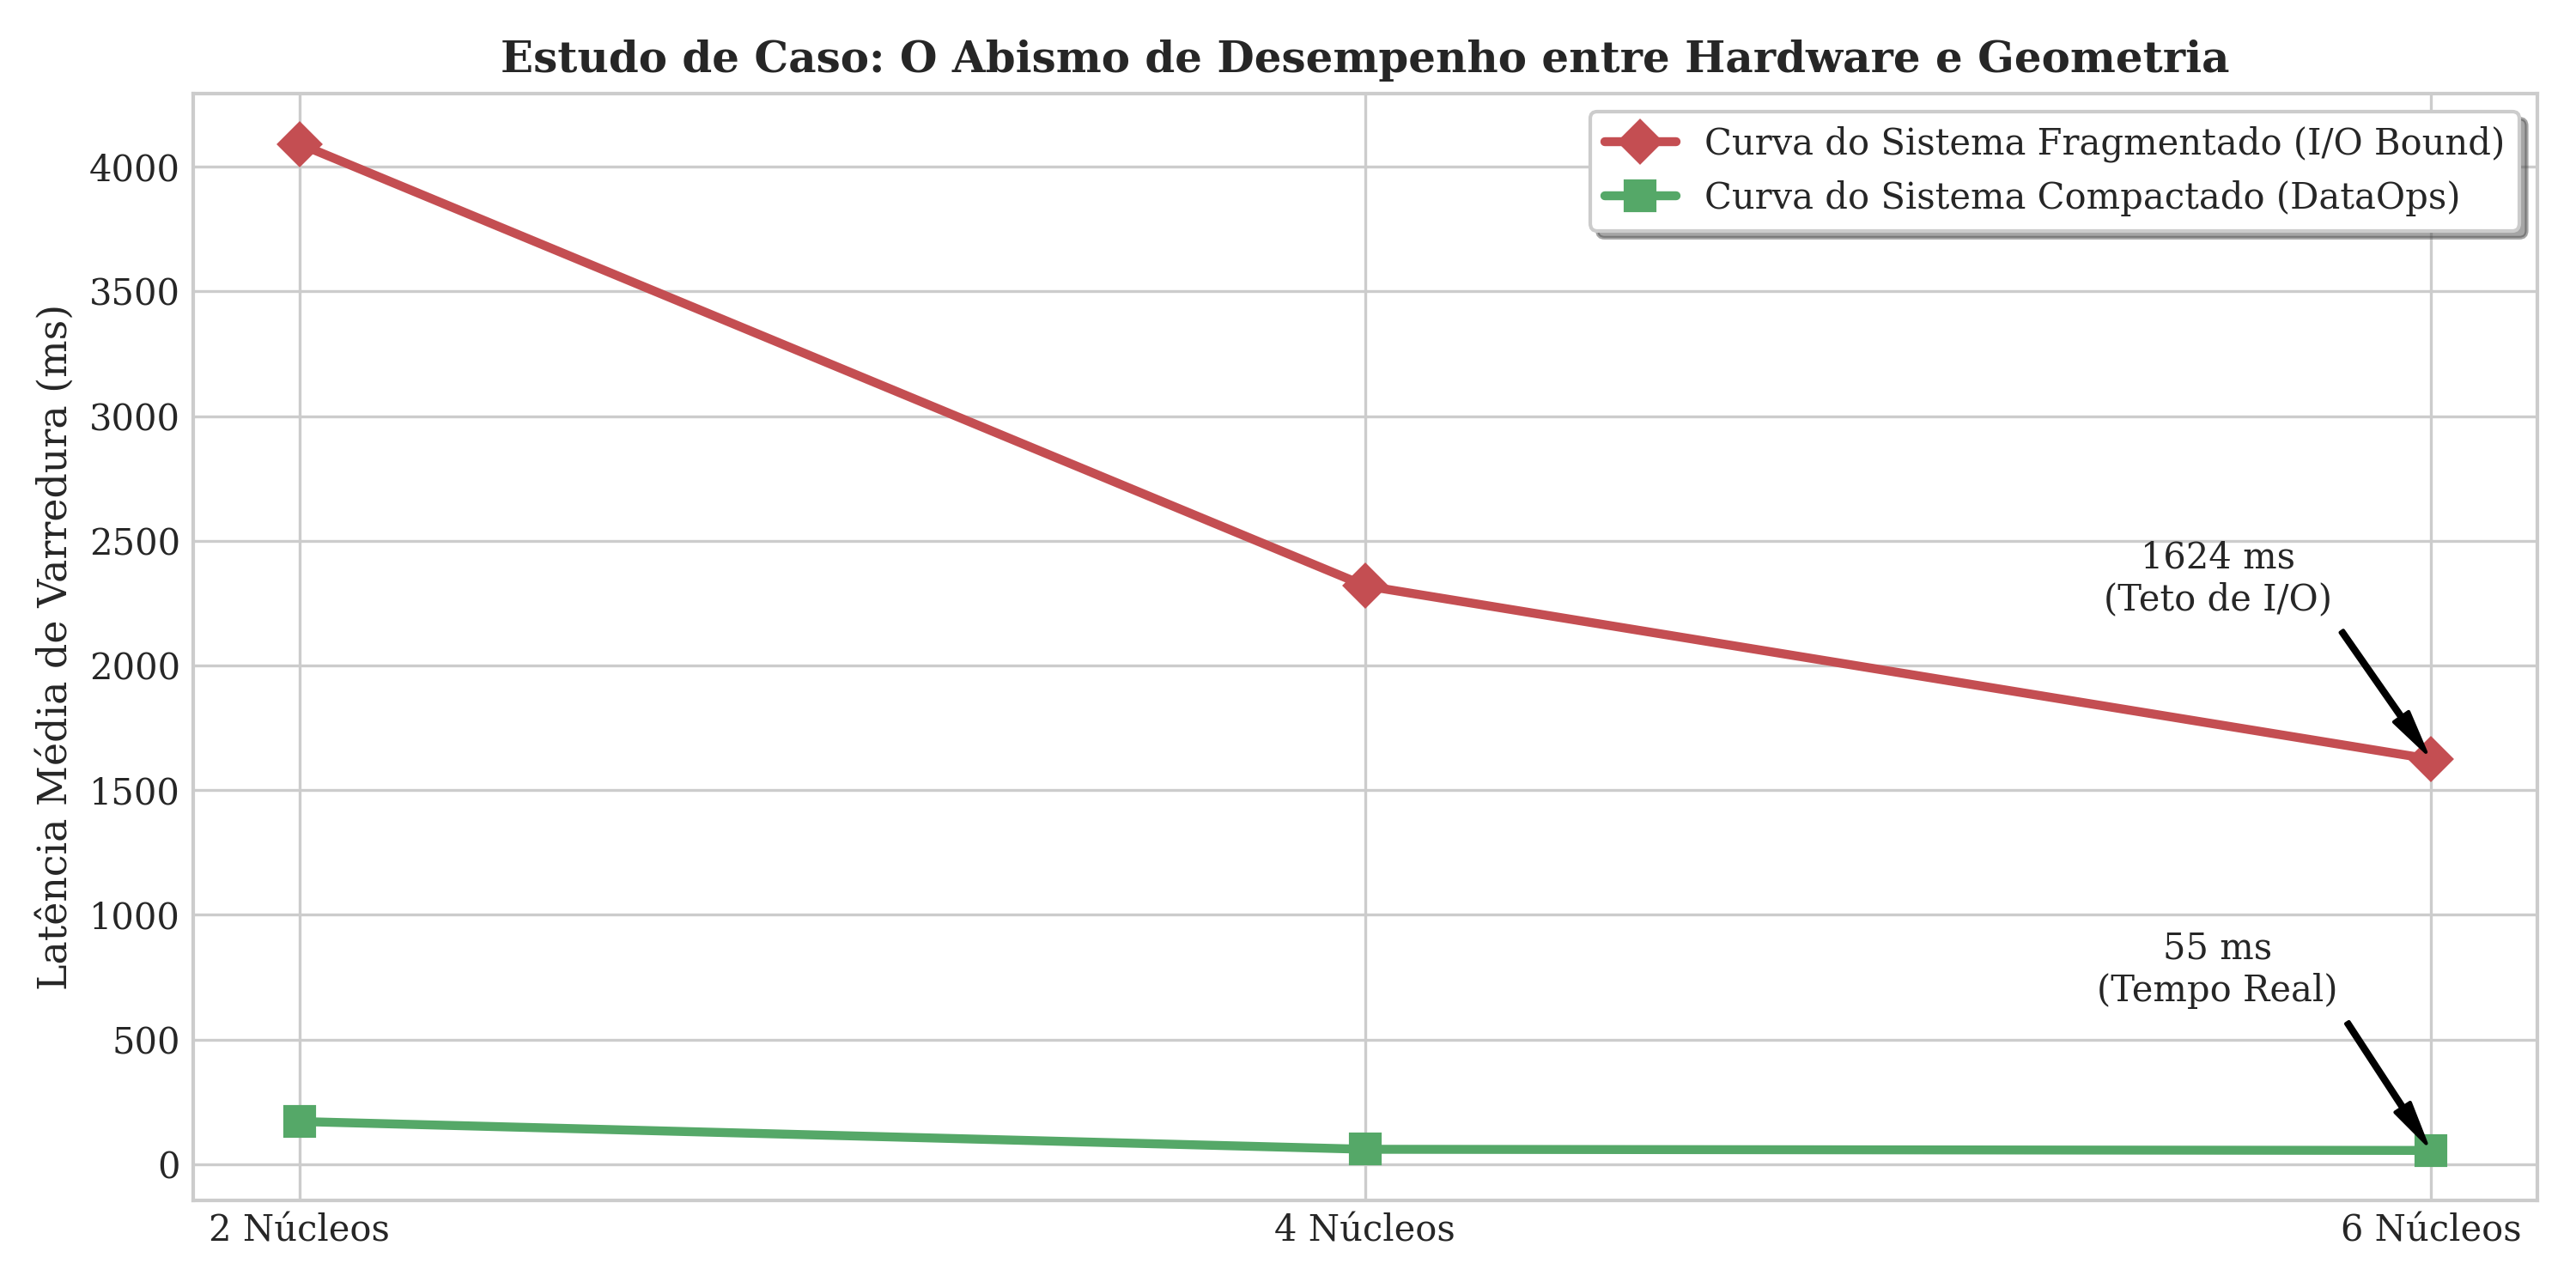
\includegraphics[width=0.85\textwidth]{materiais_apoio/figures/benchmark_preliminar/r3_comparativo_latencia_geral.png}
    \caption{Comparativo de Desempenho: Dados Fragmentados vs. Compactados.}
    \label{fig:abismo_desempenho}
\end{figure}

A Tabela \ref{tab:fator_dataops} quantifica a magnitude dessa otimização. A intervenção algorítmica revelou-se sistematicamente superior à infraestrutura física: o sistema estrangulado a 2 núcleos lendo a base compactada (171ms) foi, na prática, \textbf{\textasciitilde{}9,5 vezes} mais rápido do que o hospedeiro em potência máxima (6 núcleos) tentando processar o caos estrutural (1.624ms).

\begin{table}[H]
    \centering
    \footnotesize
    \caption{Redução de Latência Relativa por Alocação de CPU.}
    \label{tab:fator_dataops}
    \begin{tabular}{lccc}
        \toprule
        \textbf{Hardware} & \textbf{Cold Start (Frag.)} & \textbf{Cold Start (Comp.)} & \textbf{Aceleração} \\
        \midrule
        2 Núcleos & 4.092 ms & 171 ms & 23,9$\times$ \\
        4 Núcleos & 2.320 ms & 60 ms  & 38,8$\times$ \\
        6 Núcleos & 1.624 ms & 55 ms  & 29,4$\times$ \\
        \bottomrule
    \end{tabular}
\end{table}

\begin{figure}[H]
    \centering
    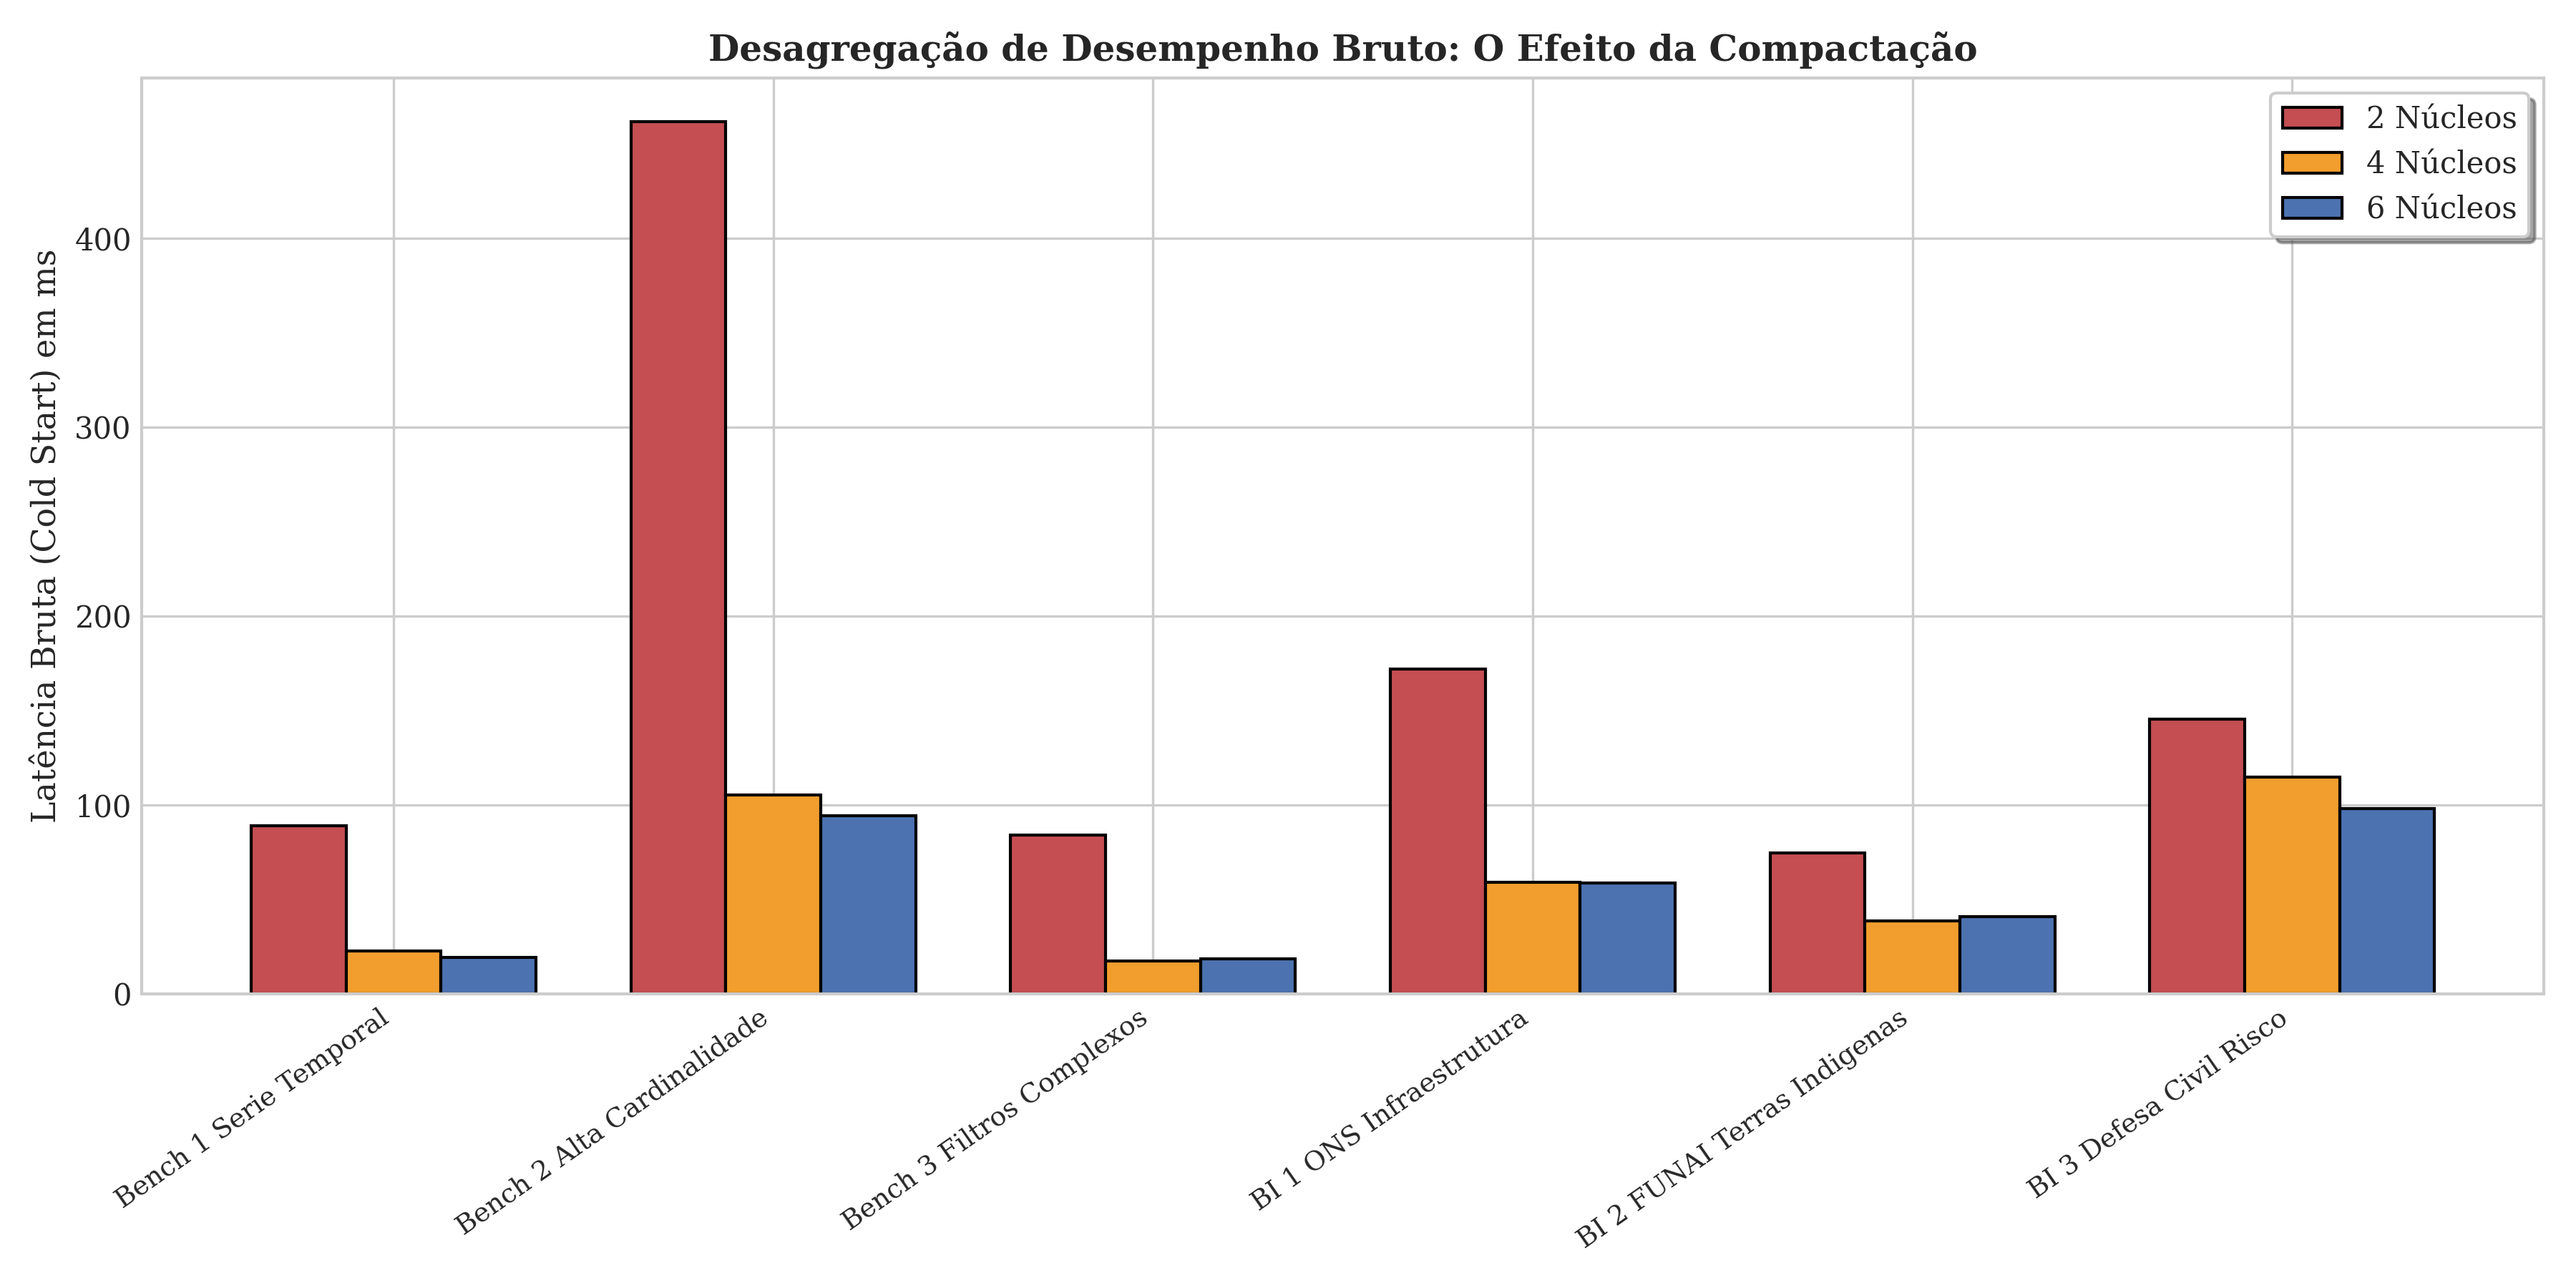
\includegraphics[width=0.85\textwidth]{materiais_apoio/figures/benchmark_preliminar/r2_latencia_por_cpu_compactado.png}
    \caption{Latência por Domínio de Consulta após Compactação (Março/2026).}
    \label{fig:barras_compactado}
\end{figure}

\subsection{Matriz de Capacidade e Saturação (Throughput)}

Embora a arquitetura básica exija escasso poder computacional (sub-100ms com 2 núcleos), a topologia \textit{Medallion} introduz alta complexidade matemática. O carregamento estrito de volumetrias da camada \textit{Silver} (e.g., polígonos GeoJSON de Terras Indígenas) desloca violentamente o gargalo sistêmico do I/O de disco para a CPU e Memória (\textit{Heap} da JVM). Para validar a resiliência estrutural a esse cenário logístico severo, executou-se a matriz de capacidade concorrente.

A avaliação atestou que a renderização de mapas analíticos sob a arquitetura empregada é primariamente \textit{CPU-Bound}. O cenário \textbf{Baseline (1.0 CPU)} apresentou degradação de desempenho logo no primeiro operador, estagnando em \textbf{0,89 QPS} com falha em 42,7\% das requisições (\textit{Timeouts}). Isso atesta que um núcleo solitário não sustenta a alta carga de alocação de memória exigida pelos \textit{Lookups} dimensionais (que transferem as volumosas matrizes GeoJSON, previamente cruzadas na camada Silver pelo Python, para o \textit{Heap} do Druid).

Em contrapartida, a alocação expandida no cenário \textbf{Query Heavy (2.0 CPU)} demonstrou resiliência operacional. O sistema escalou a vazão (\textit{Throughput}) de forma constante, suportando até 16 \textit{threads} simultâneas e formando um platô sustentável na marca de \textbf{\textasciitilde{}2,0 QPS}. Nesse estado resiliente, novas conexões aguardam em fila, mas são integralmente entregues sem geração de \textit{Timeouts HTTP 500} (0\% de erro).

Nota-se, contudo, a presença eventual de \textit{outliers} negativos na curvatura de vazão linear. Em pontos específicos da escalada da carga, o sistema sofreu quedas abruptas de vazão em janelas milissegundares. Levanta-se a forte hipótese técnica de que este comportamento anômalo remeta a pausas prolongadas de \textit{Garbage Collection} (GC \textit{Stop-The-World}) e a eventos de \textit{Thread Contention}, embora essa suposição exigisse medições com \textit{profilers} ativos na JVM para constatação isolada.

\begin{figure}[H]
    \centering
    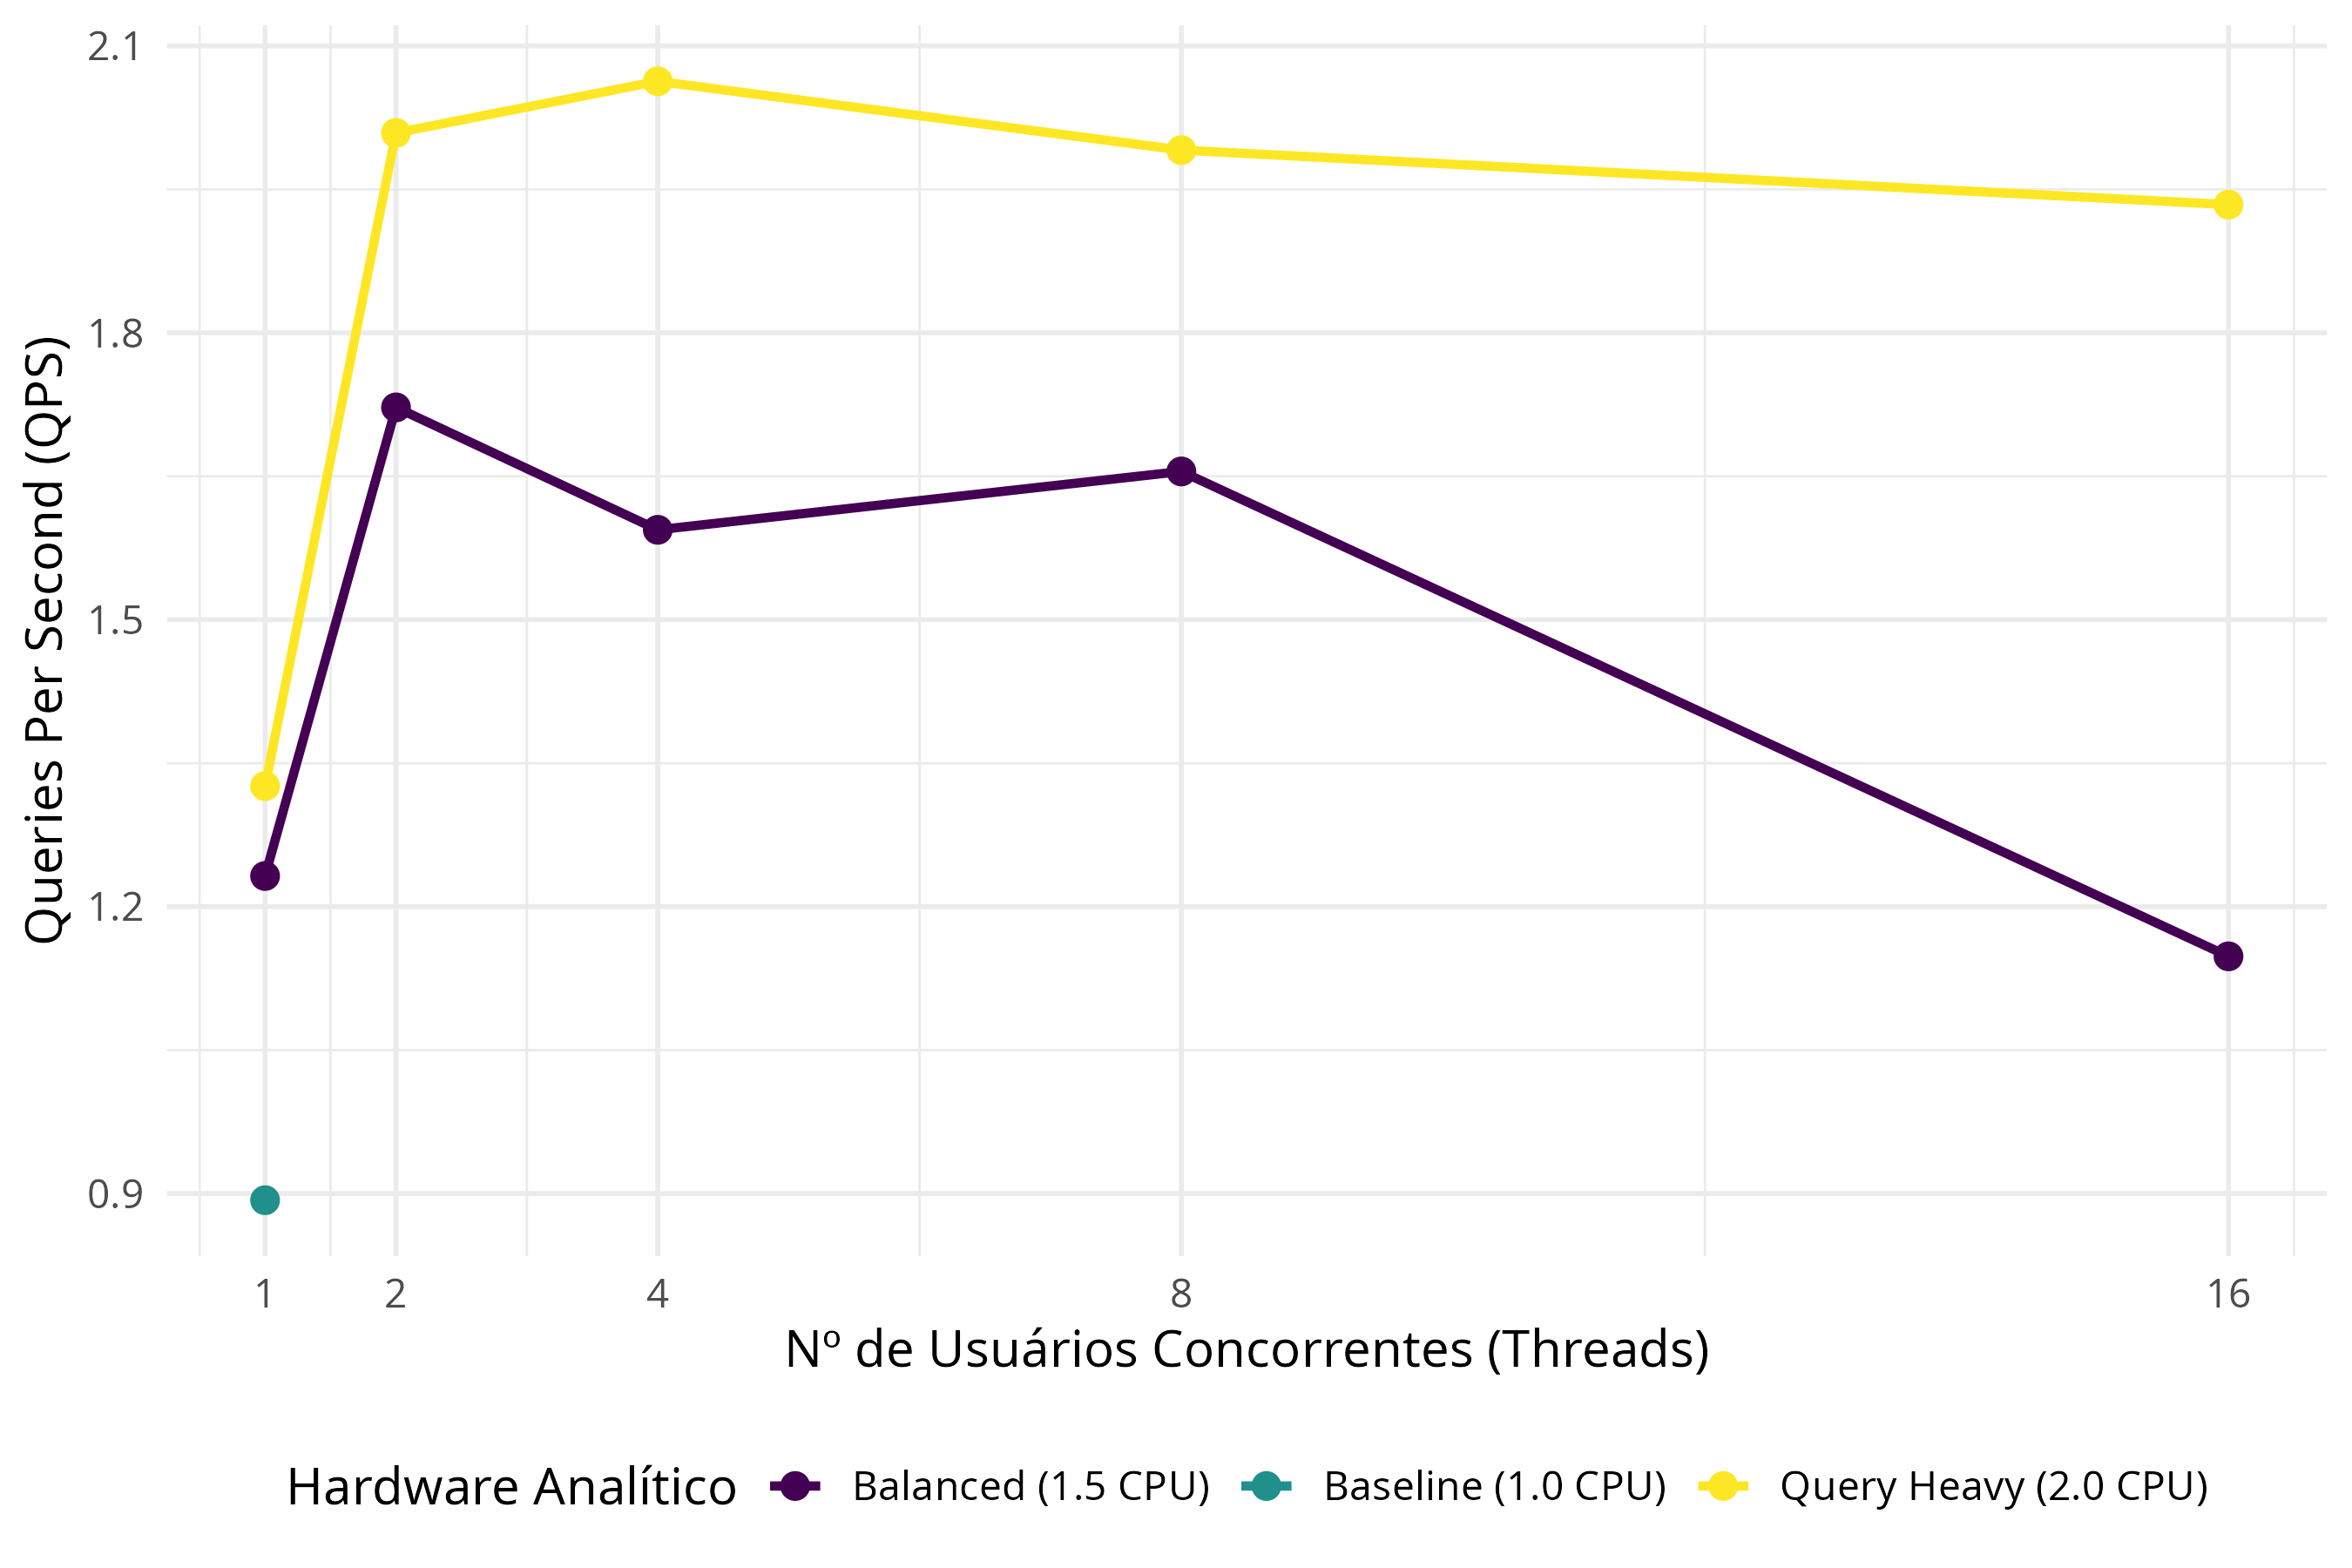
\includegraphics[width=0.8\textwidth]{analise_R/plots/qps_saturation_new.png}
    \caption{Vazão Analítica (QPS) por Perfil de Escalabilidade.}
    \label{fig:qps_saturation}
\end{figure}

\subsection{Explosão de Latência e Percentil 95 (P95)}

Conforme demonstrado estatisticamente, no cenário \textit{Baseline} a latência e o volume de falhas descontrolaram-se já no primeiro operador em rede. Em contraste, o cenário \textit{Query Heavy} absorveu o impacto geométrico sem gerar interrupções, contendo a latência P95 na faixa aceitável de \textbf{\textasciitilde{}2,8 segundos} (com 2 operadores) até o limiar de \textbf{\textasciitilde{}8,2 segundos} sob o estresse de 8 operadores processando agregações massivas simultaneamente.

Contudo, fora da curva de 95\% (\textit{outliers}), registraram-se picos de latência. Esses engasgos ocorrem quando cruzamentos espaciais densos (e.g., sobreposição espacial em Terras Indígenas) esgotam a memória \textit{Heap} da JVM e os \textit{Merge Buffers}, forçando pausas prolongadas de \textit{Garbage Collection} (GC). Ressalta-se que tais anomalias foram induzidas por \textit{queries} puramente de estresse (sem amarras temporais). Na operação real do SIRDA, filtros de temporalidade (ex: janela crítica de 7 dias) impedem que um pacote GeoJSON dessa magnitude congestione a memória em uma única requisição.

\begin{figure}[H]
    \centering
    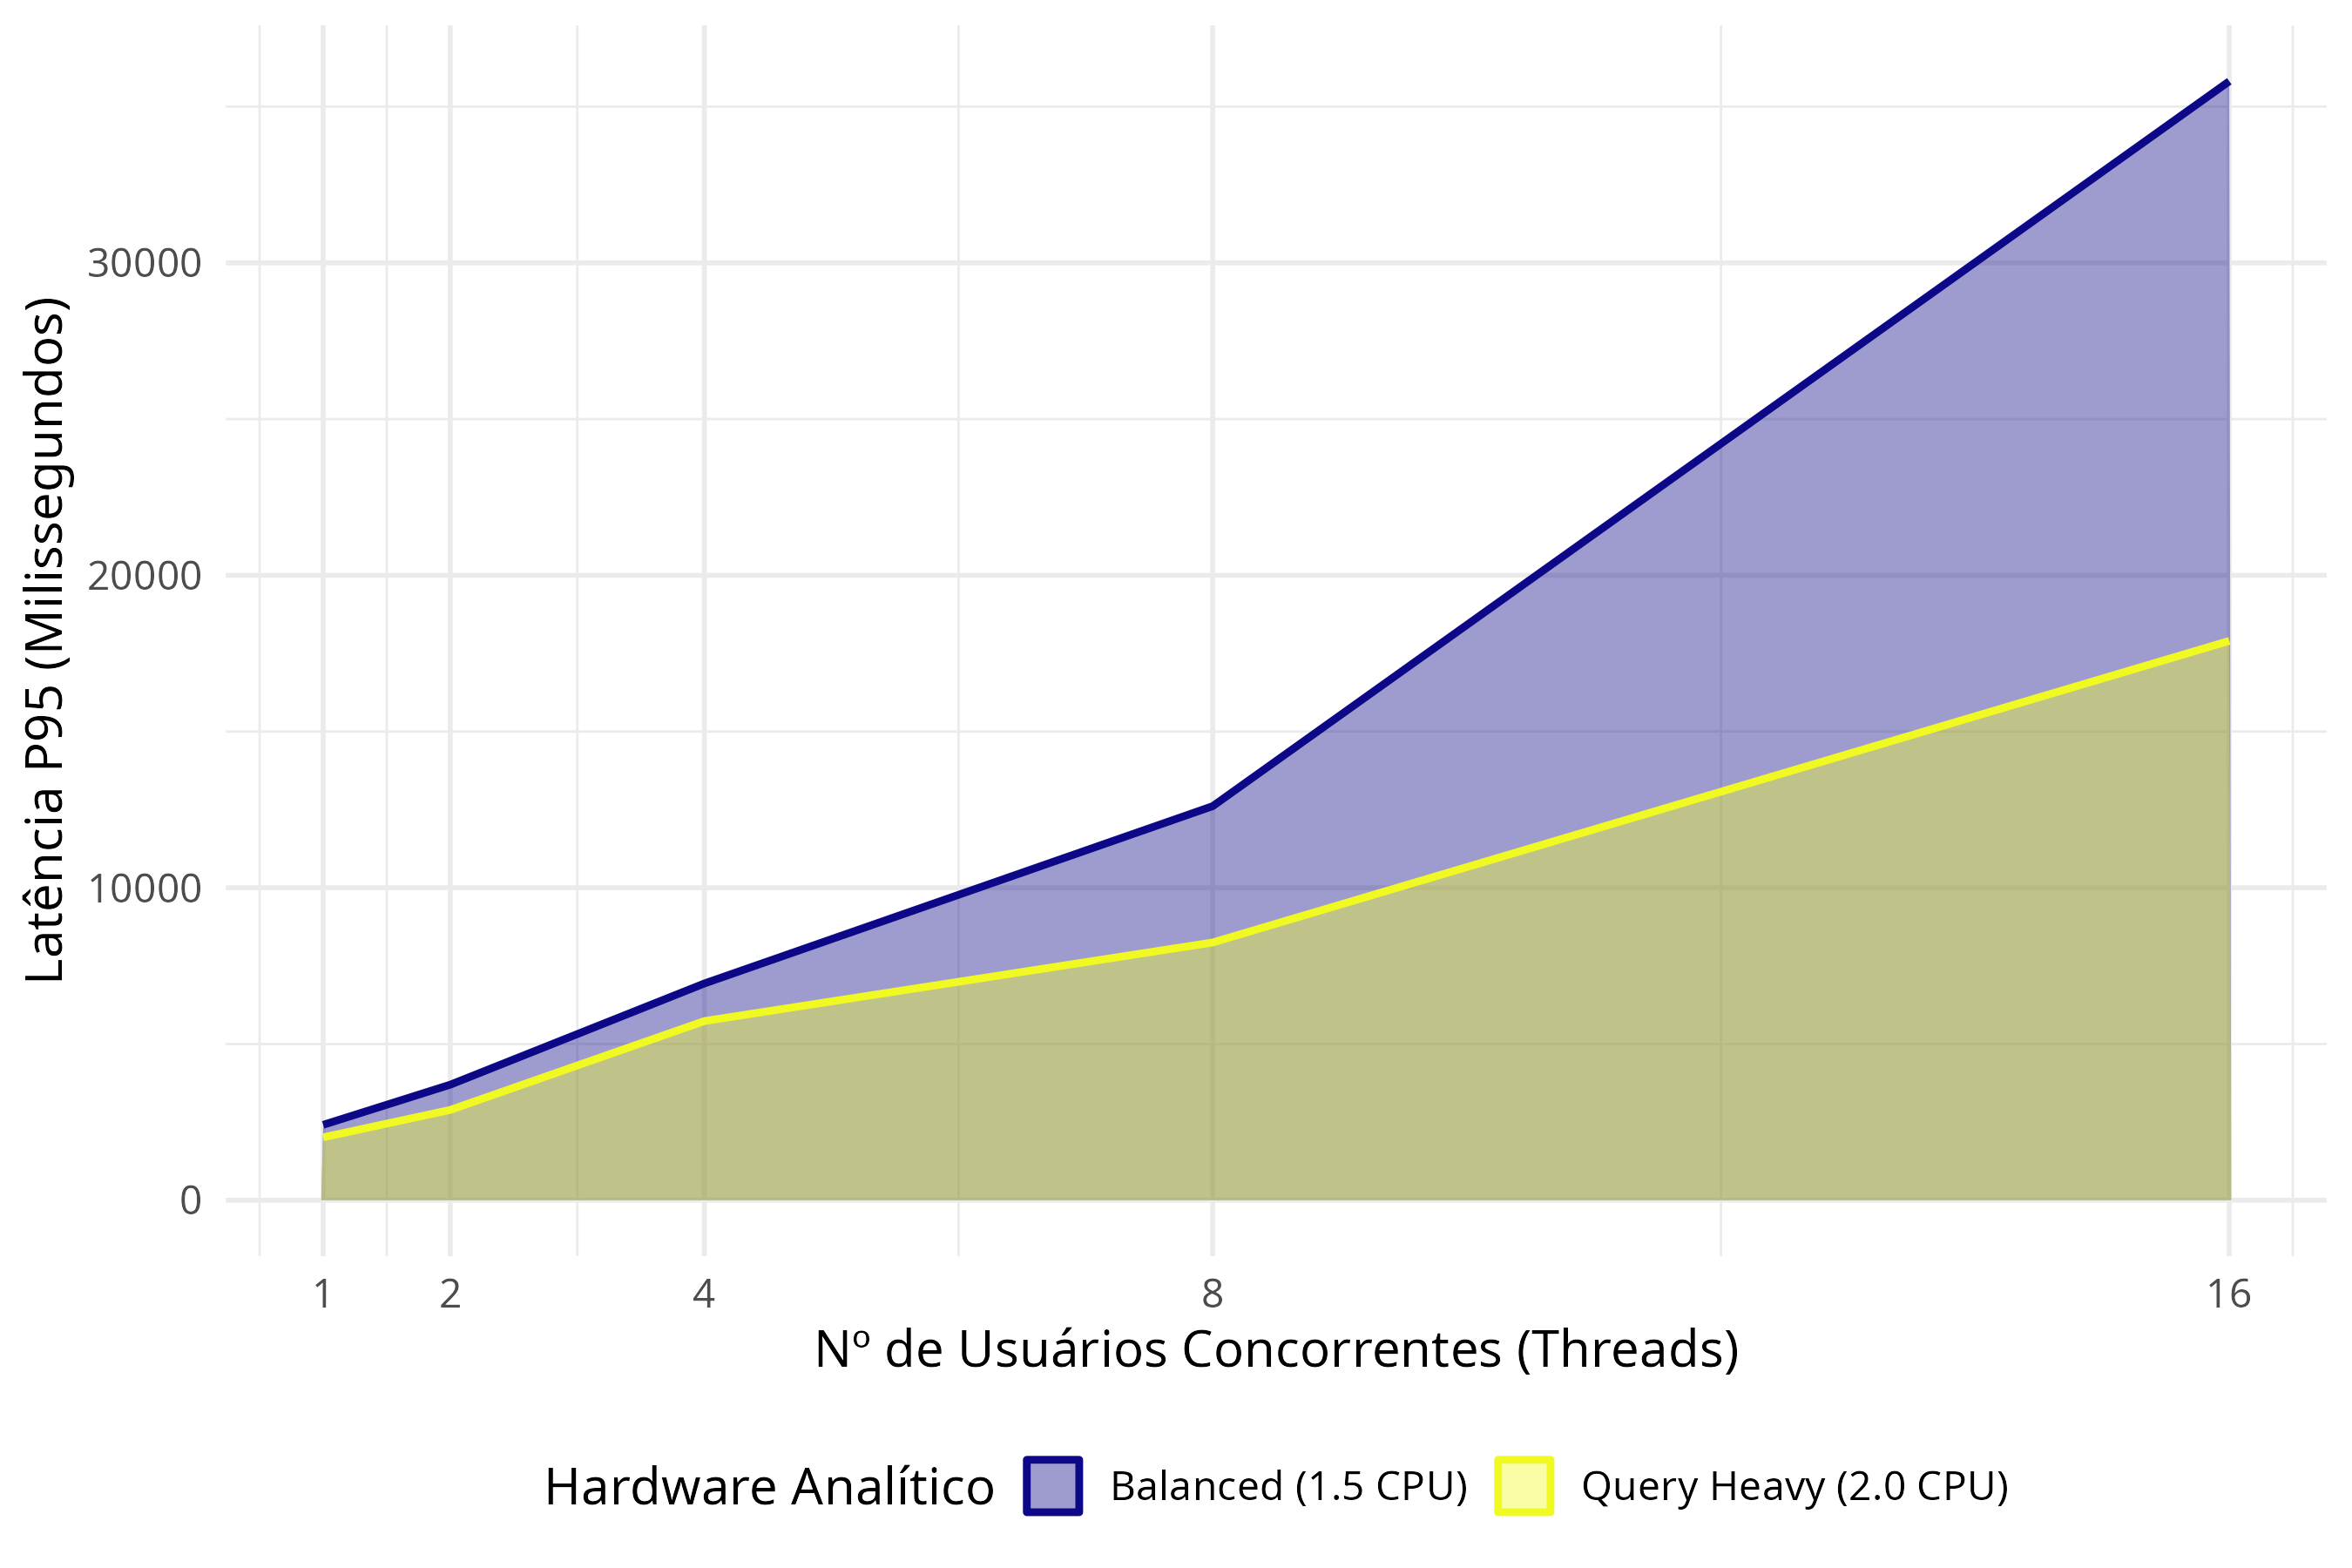
\includegraphics[width=0.8\textwidth]{analise_R/plots/p95_latency_new.png}
    \caption{Degradação de Latência (P95) durante Escalonamento.}
    \label{fig:p95_latency}
\end{figure}

\subsection{Eficiência do Mecanismo de Cache de Memória}

No contexto operacional da plataforma SIRDA, painéis gerenciais (\textit{Dashboards}) promovem uma forte redundância de consultas similares por diferentes operadores. O mecanismo nativo de intercepção (\textit{Broker Query Cache}) provou atuar mitigando a debilidade da restrição de processamento de núcleo.

Pela ótica da escala logarítmica representada, as requisições puras ao disco e aos segmentos de dados (\textit{Cold Start}) operam em densidades predominantemente acomodadas acima de $10^3$ (1.000 a 10.000 milissegundos). Por sua vez, o acerto de memória (\textit{Warm Start}) reduz drasticamente a latência para faixas abaixo de $10^2$ (sub-100 milissegundos), garantindo que metade da atividade analítica pesada seja entregue numa magnitude de quase tempo real e economizando leituras nos índices colunares subjacentes (\textit{Bitmap Indexes}).

A base matemática exibiu extensões esguias persistentes no violino de aquecimento (caudas longas no cenário \textit{Warm}), atestando instantes em que requisições repetidas demoraram o mesmo ou até mais tempo que requisições originais em disco. A hipótese analítica primária para este fenômeno de \textit{outliers} recai sobre a ocorrência de \textit{Cache Eviction} sistêmico. Sob carga frenética e concorrente, postula-se que o vetor local de memória do \textit{Broker} lota precocemente de dados variados, sendo forçado a "despejar" (remover) painéis outrora armazenados.

\begin{figure}[H]
    \centering
    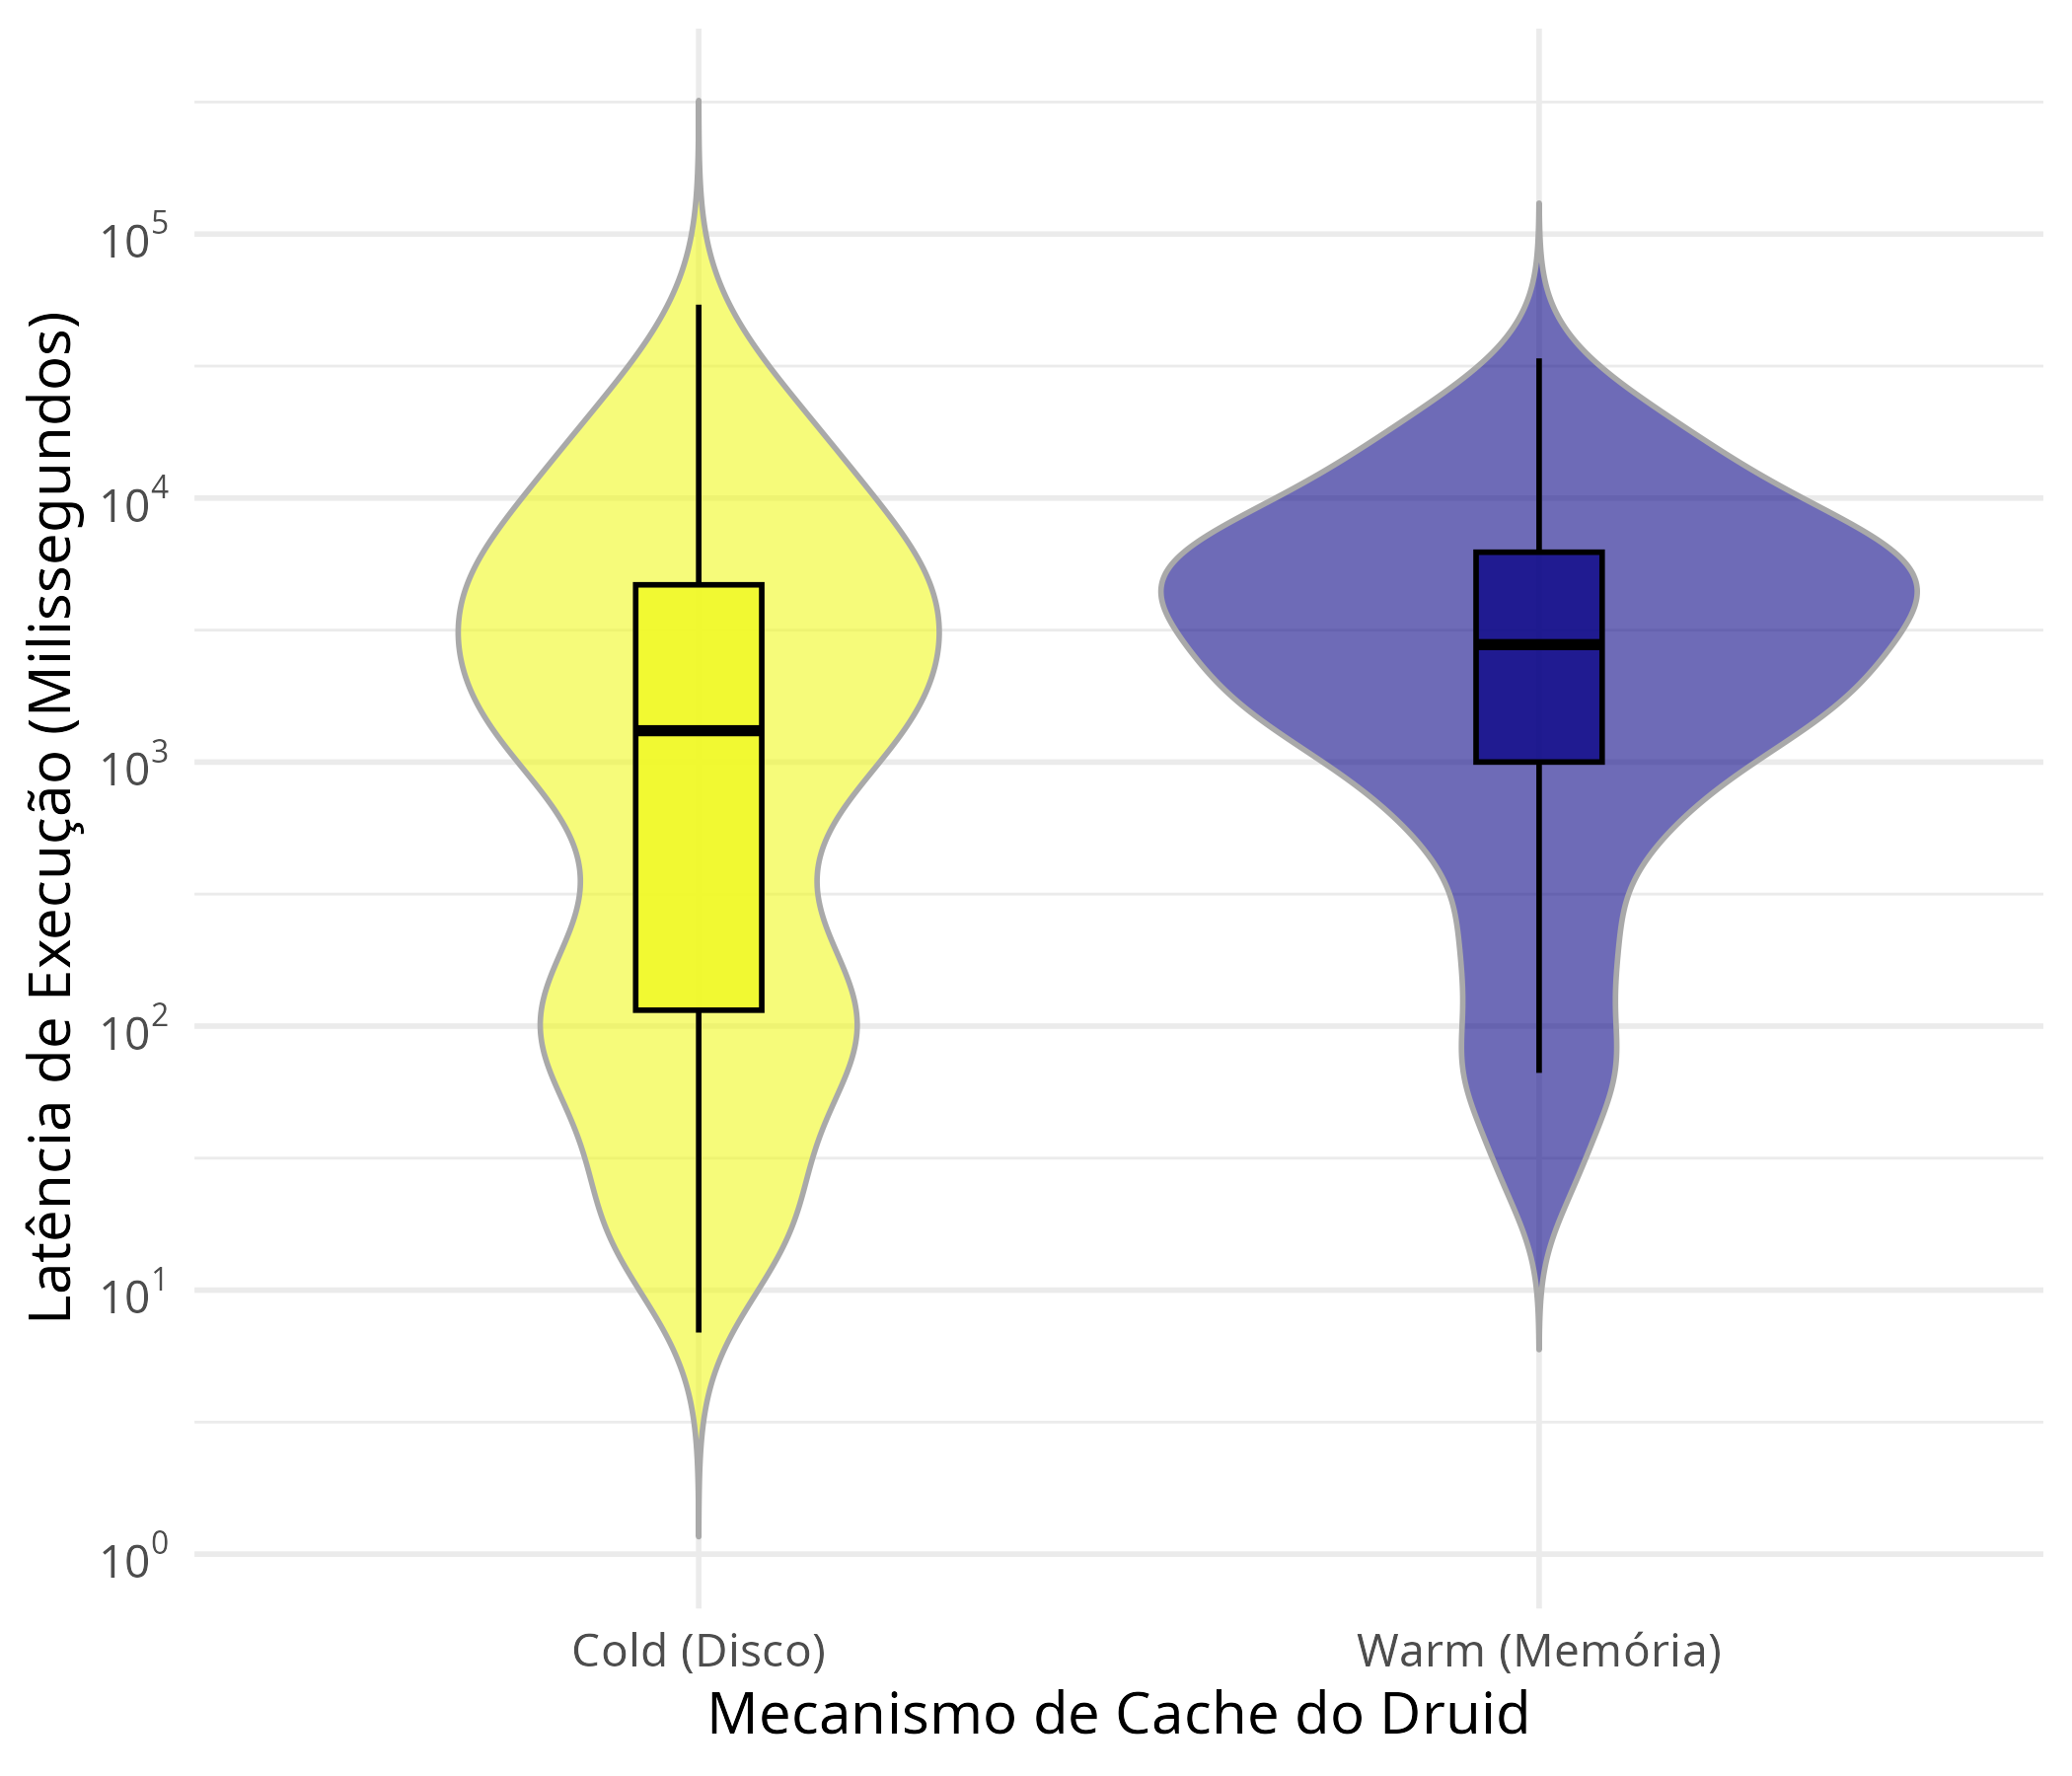
\includegraphics[width=0.8\textwidth]{analise_R/plots/cache_violin_new.png}
    \caption{Distribuição de Latência: Cache vs. Leitura Nativa.}
    \label{fig:cache_efficiency}
\end{figure}

\subsection{Consumo Físico de Contêineres e Esgotamento (Memory Footprint)}

A série temporal corrobora a estabilidade dos nós conteinerizados perante o limite estrito do \textit{Cgroup} (Docker), demonstrando teto rígido (inferior a 90\%) e atestando a ausência de vazamento de memória (\textit{Memory Leak}). O motor de varredura (\textit{Historical}) acomoda-se em platôs seguros (70\%-80\%) durante as rajadas de carga.

De maneira análoga, o contêiner integrador (\textit{Broker}) exibe um comportamento resiliente, evidenciando que grandes cargas cartográficas em memória (GeoJSON) são velozmente serializadas, com espaço recuperado pelas rotinas de limpeza da JVM (\textit{Garbage Collection}). Sem o registro de falhas por esgotamento (\textit{OOM Killed}), conclui-se que o verdadeiro gargalo analítico da plataforma reside no processamento matemático espacial (restrição de vCPU), e não na escassez de RAM.

\begin{figure}[H]
    \centering
    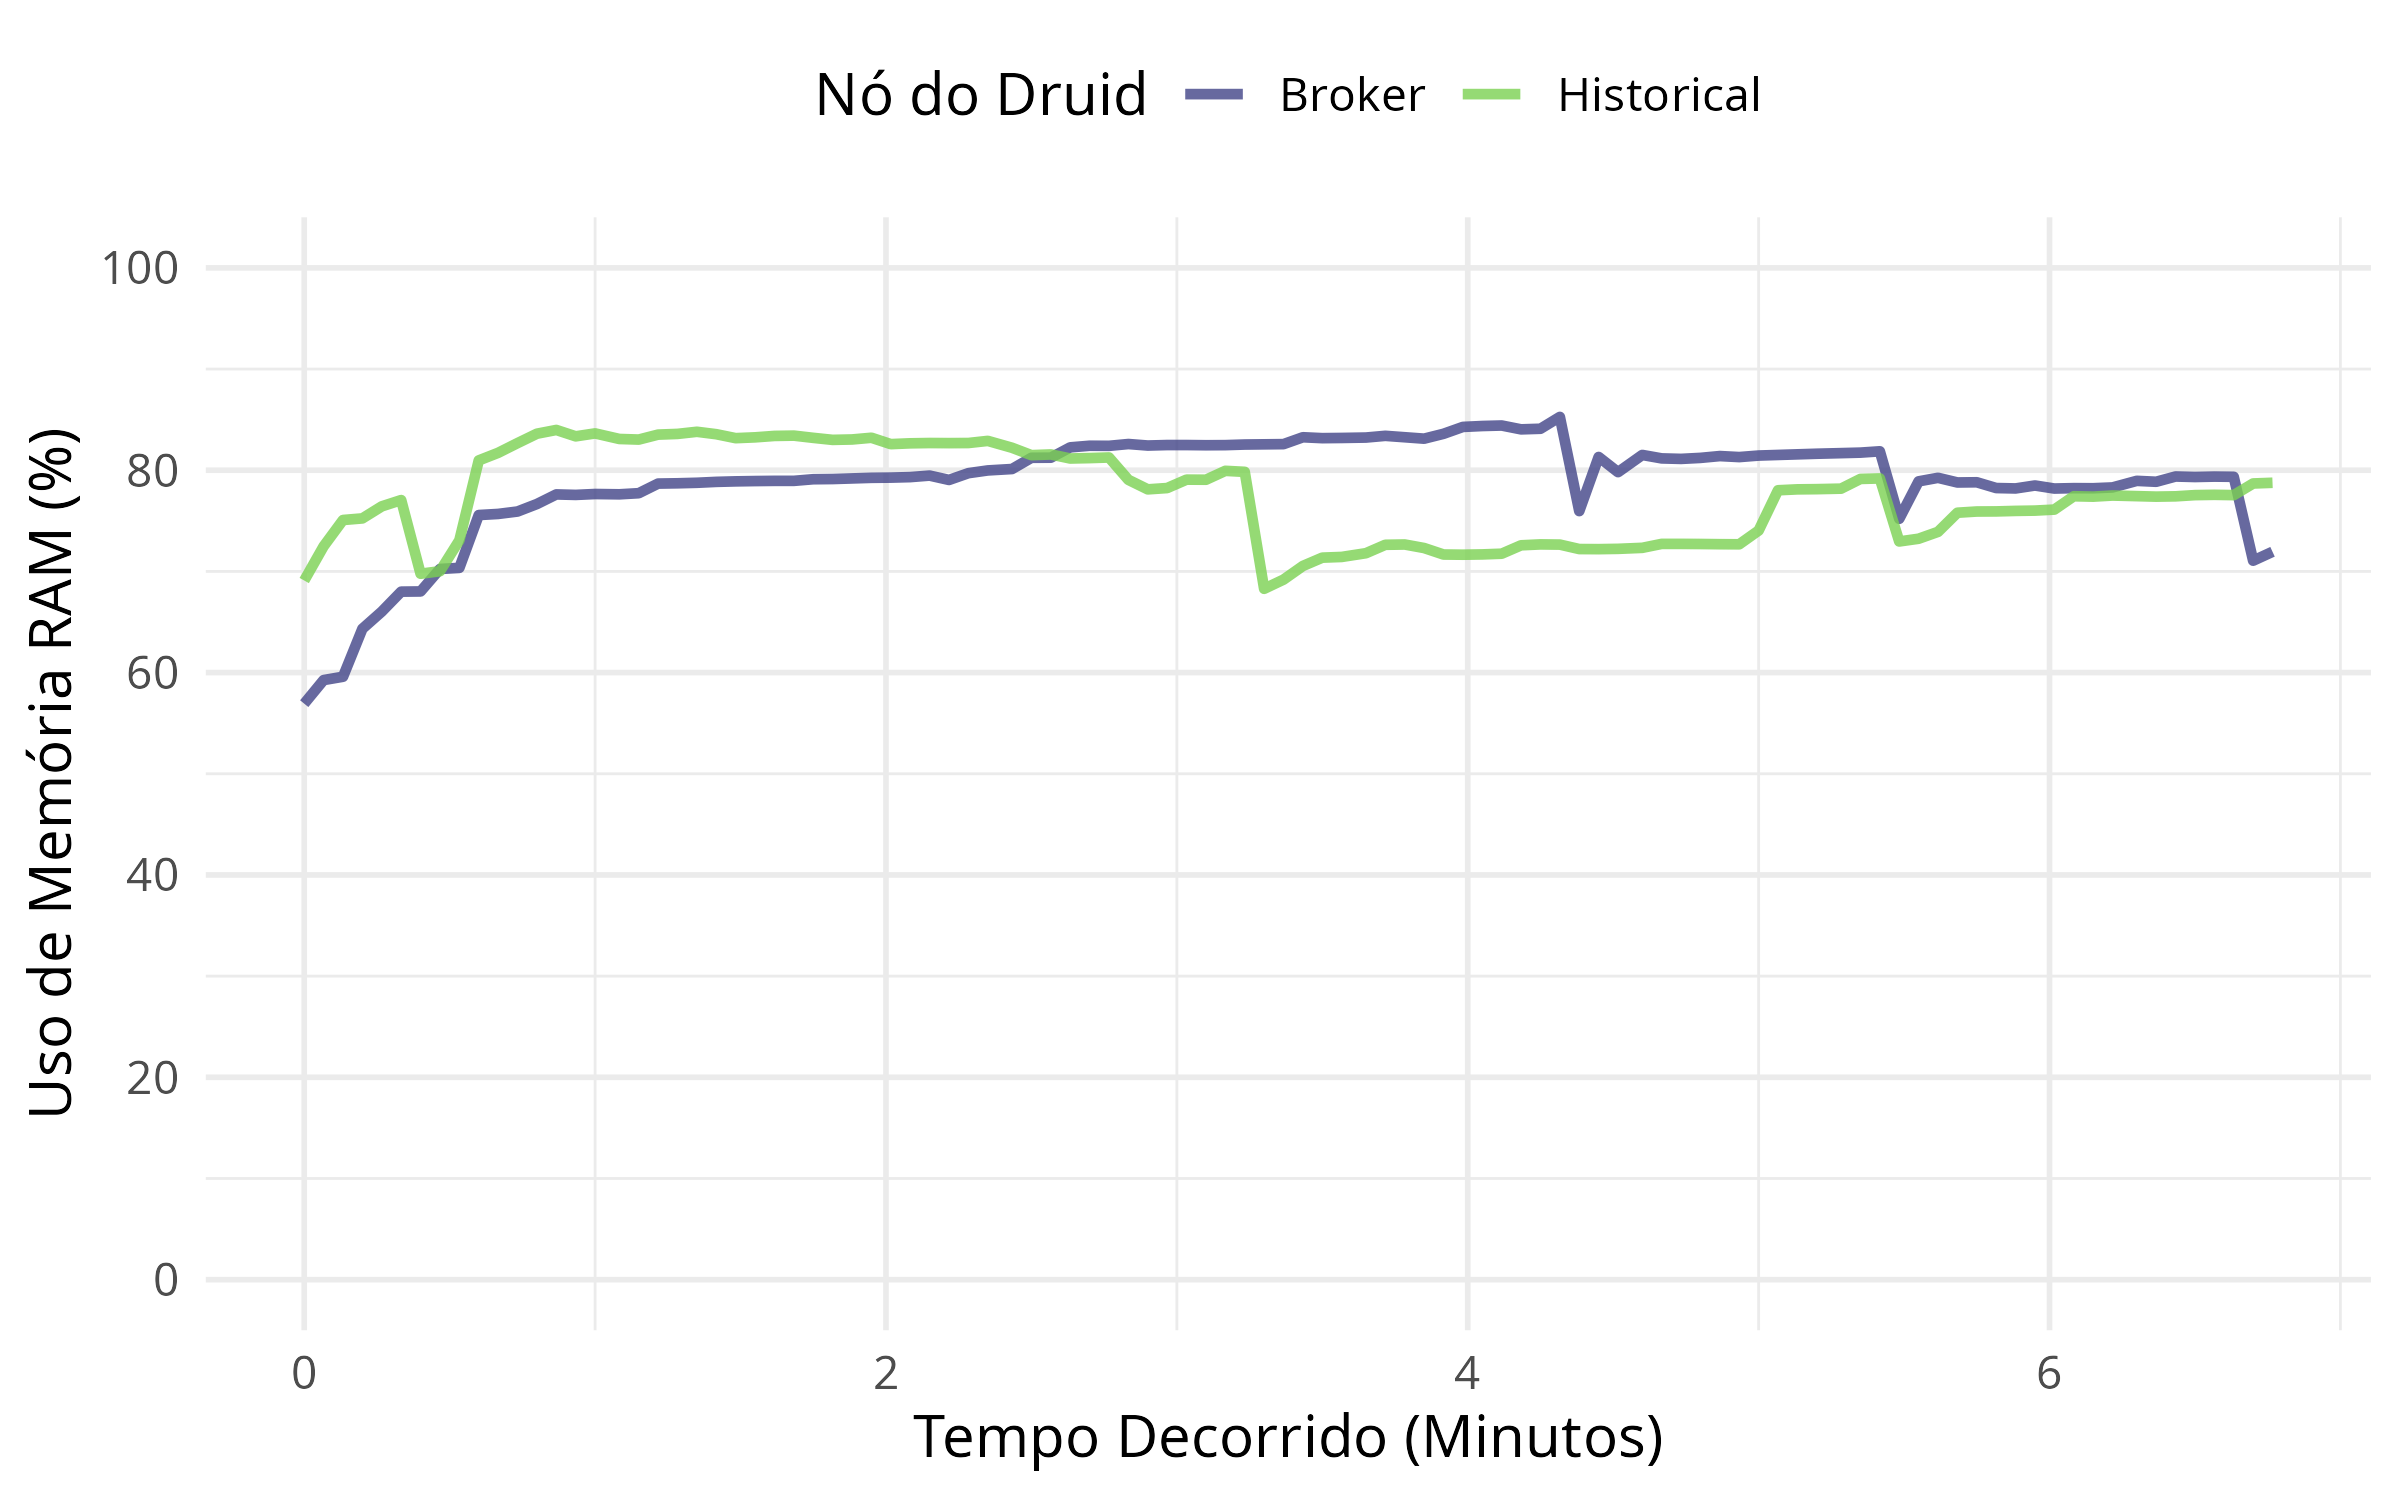
\includegraphics[width=0.8\textwidth]{analise_R/plots/ram_usage_new.png}
    \caption{Oscilação do Consumo de RAM no Apache Druid.}
    \label{fig:ram_usage}
\end{figure}

\subsection{Análise Operacional do Cenário de Crise Ambiental (2025)}

Após a otimização arquitetural, a plataforma foi submetida a um cenário extremo de estiagem e incêndios florestais baseados no monitoramento de anomalias térmicas via sensoriamento remoto \cite{giglio_modis_2016}. O sistema permitiu transformar o volume massivo de biometria de calor crua (\textit{raw fire points}) em inteligência tática aplicável à infraestrutura nacional.

\subsubsection{Panorama Geral e Dinâmica nos Biomas}

A crise ambiental atingiu o território nacional de forma aguda e irregular. A Figura \ref{fig:dashboard_outubro} ilustra um painel analítico focado na amostra de outubro de 2025 (pico da estiagem), evidenciando os focos ativos, a área destruída e a severidade do evento (FRP). O painel atesta a macro-evolução do desastre, marcada por um comportamento escalonado e contínuo impulsionado pelo acúmulo agudo das condições de seca.

\begin{figure}[H]
    \centering
    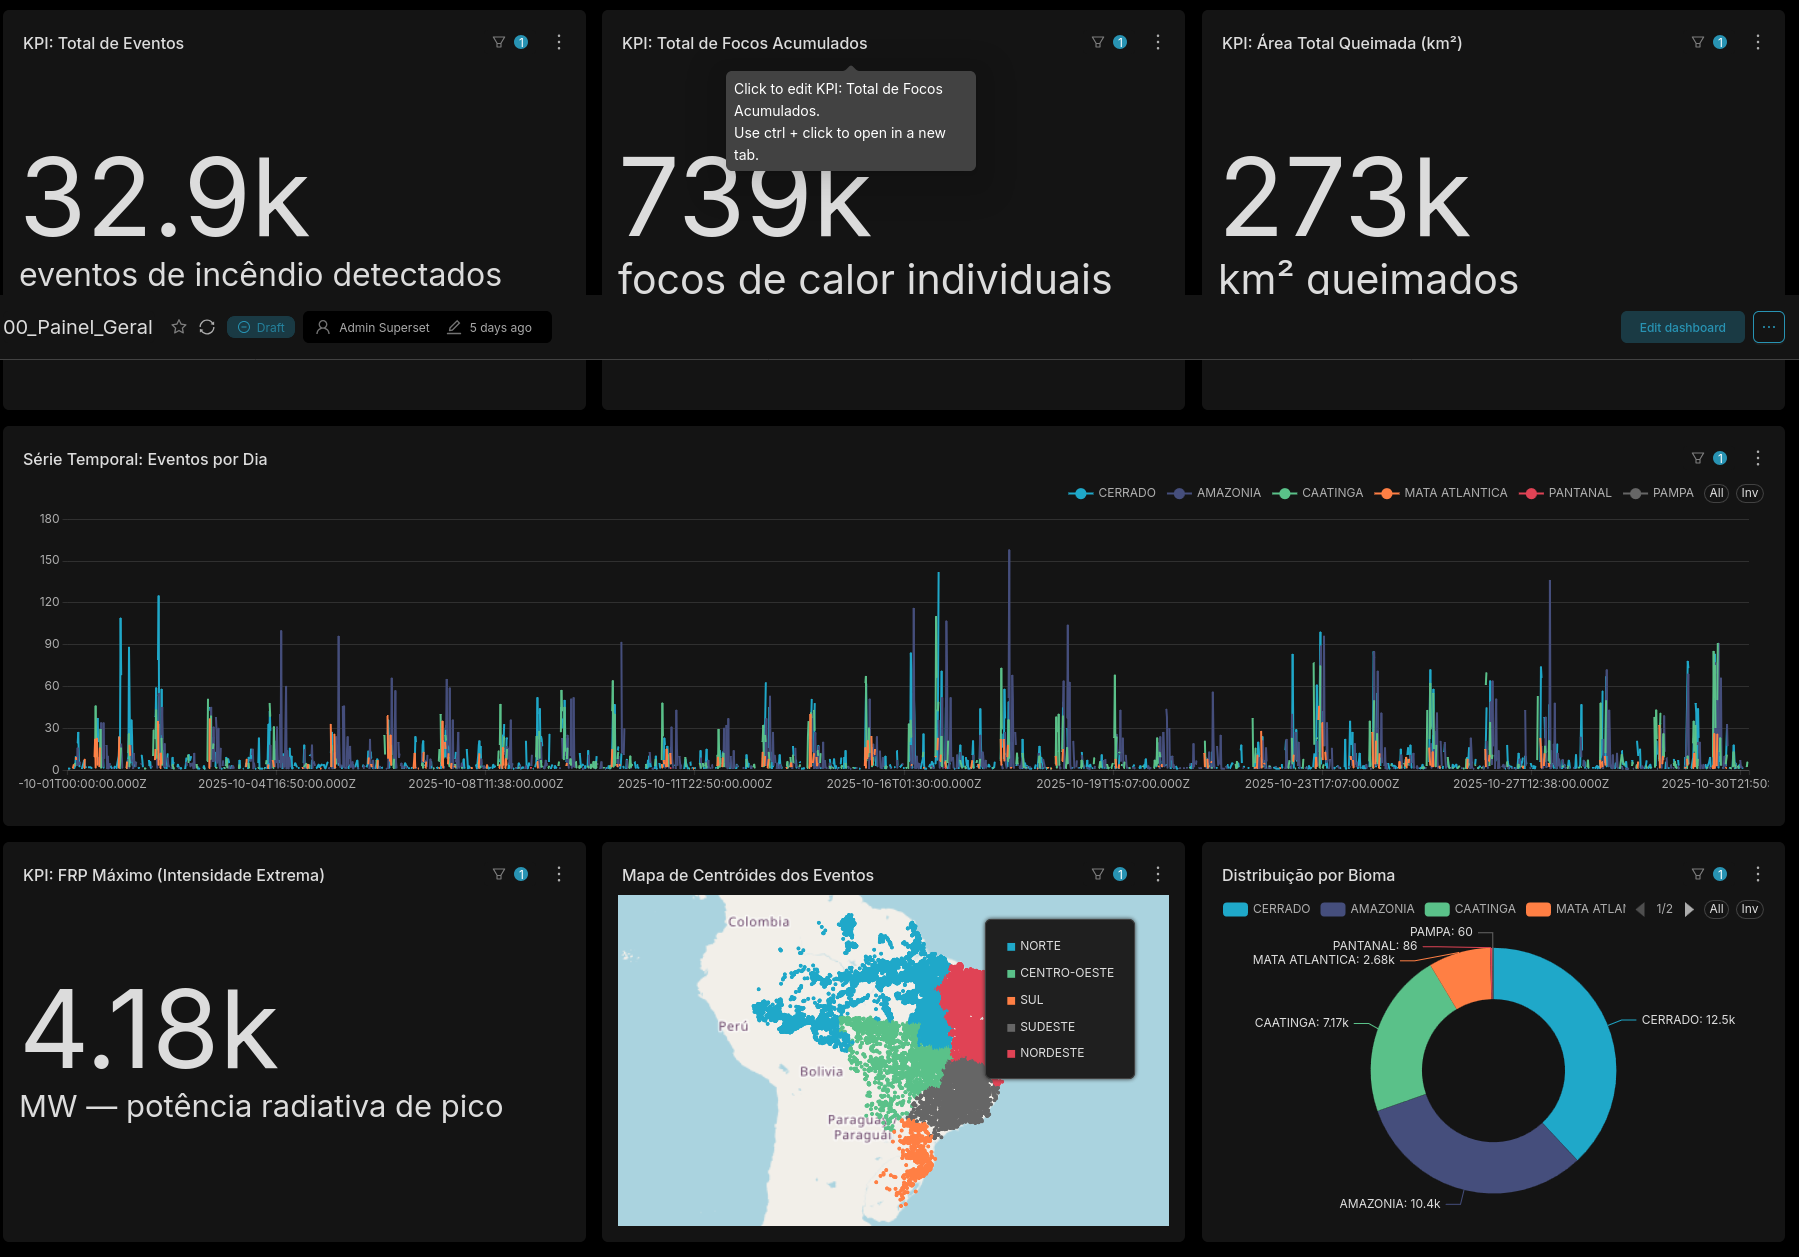
\includegraphics[width=0.9\textwidth]{materiais_apoio/figures/DashBoard.png}
    \caption{Visualização Analítica de Ignições (Apache Superset).}
    \label{fig:dashboard_outubro}
\end{figure}

\subsubsection{Impacto em Comunidades Vulneráveis: Terras Indígenas}

Uma das principais premissas táticas foi mensurar o nível de ameaça sistêmica às comunidades originárias utilizando as malhas poligonais oficiais da FUNAI. O motor analítico rastreou com precisão o cruzamento físico e a aproximação marginal (buffers) das coordenadas de fogo sobre essas demarcações. O resultado prático consolidou um ranking geoespacial de pressão social exibido na Figura \ref{fig:ranking_tis}, revelando os territórios indígenas que apresentaram alta vulnerabilidade espacial.

\begin{figure}[H]
    \centering
    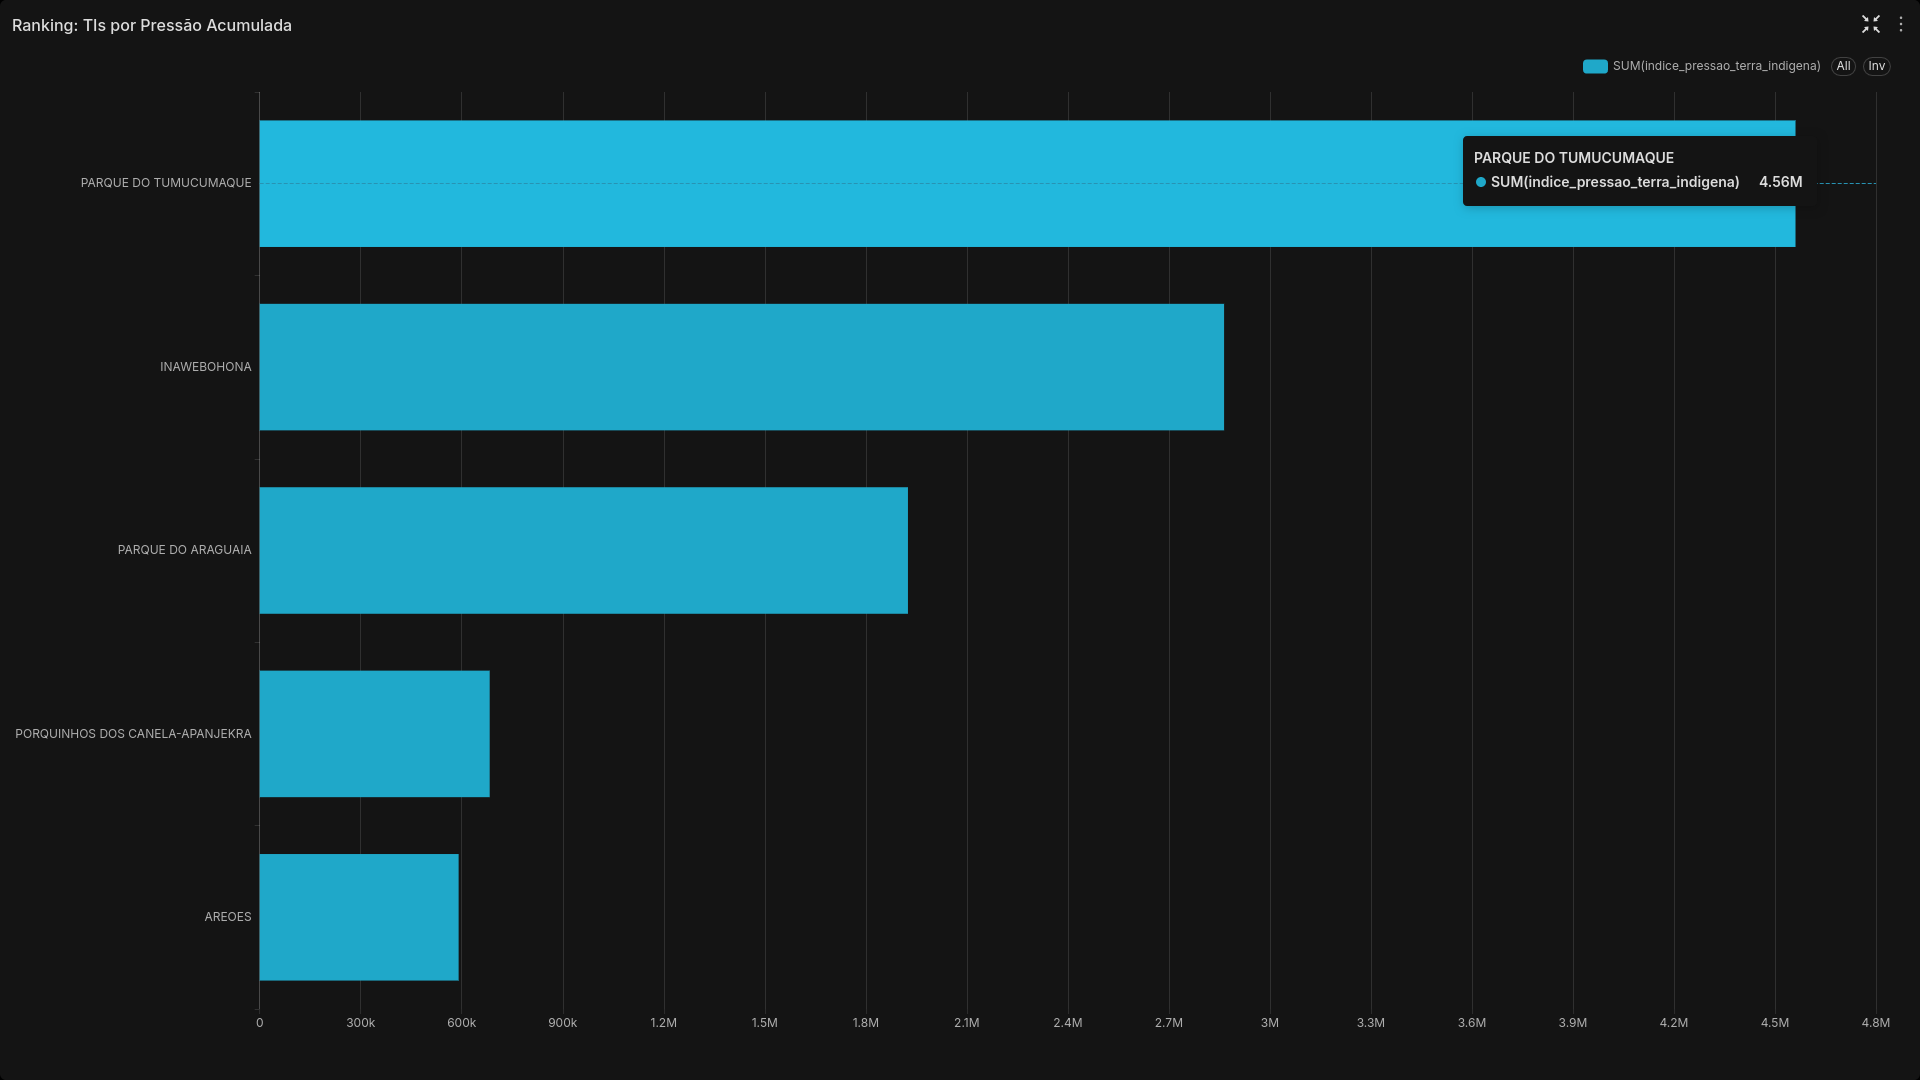
\includegraphics[width=0.9\textwidth]{materiais_apoio/figures/PressãoIndigena.png}
    \caption{Volumetria de Focos em Terras Indígenas.}
    \label{fig:ranking_tis}
\end{figure}

A agregação analítica classificou a \textbf{Terra Indígena Parque do Araguaia} (Formoso do Araguaia/TO) no 3º lugar do ranking de vulnerabilidade com base nos dados de 2025. Levanta-se a hipótese de que essa elevada concentração de anomalias térmicas reflita o avanço do pólo agroindustrial para a porção sul da Ilha do Bananal. Embora o índice calculado não determine causalidade direta para eventos isolados, as métricas parecem corroborar a narrativa cíclica de degradação na região. Segundo reportagem do portal G1, em setembro de 2026, um novo incêndio destruiu 38 residências na Aldeia Canoanã, inserida na mesma demarcação \cite{g1_canoana_2026}. A identificação prévia deste território no topo do ranking sugere que a plataforma pode atuar como um instrumento de apoio para o mapeamento de tendências de exposição e subsidiar ações preventivas.

\subsubsection{Ameaça à Infraestrutura Crítica: Setor Elétrico e Saúde (SUS)}

A integração central do projeto foi materializada na intersecção veloz entre as medições dos satélites termais e a infraestrutura civil mapeada. Centros hospitalares localizados nos arredores dos epicentros rurais de incêndio sofreram o reflexo primário de densas massas regionais de fumaça, gerando alto impacto na região de cobertura das unidades de saúde. O controle exibido na Figura \ref{fig:hospitais_criticos} rastreou não apenas o quantitativo, mas a intensidade da radiação (FRP) sobrepostas às coordenadas do Cadastro Nacional de Estabelecimentos de Saúde (CNES).

\begin{figure}[H]
    \centering
    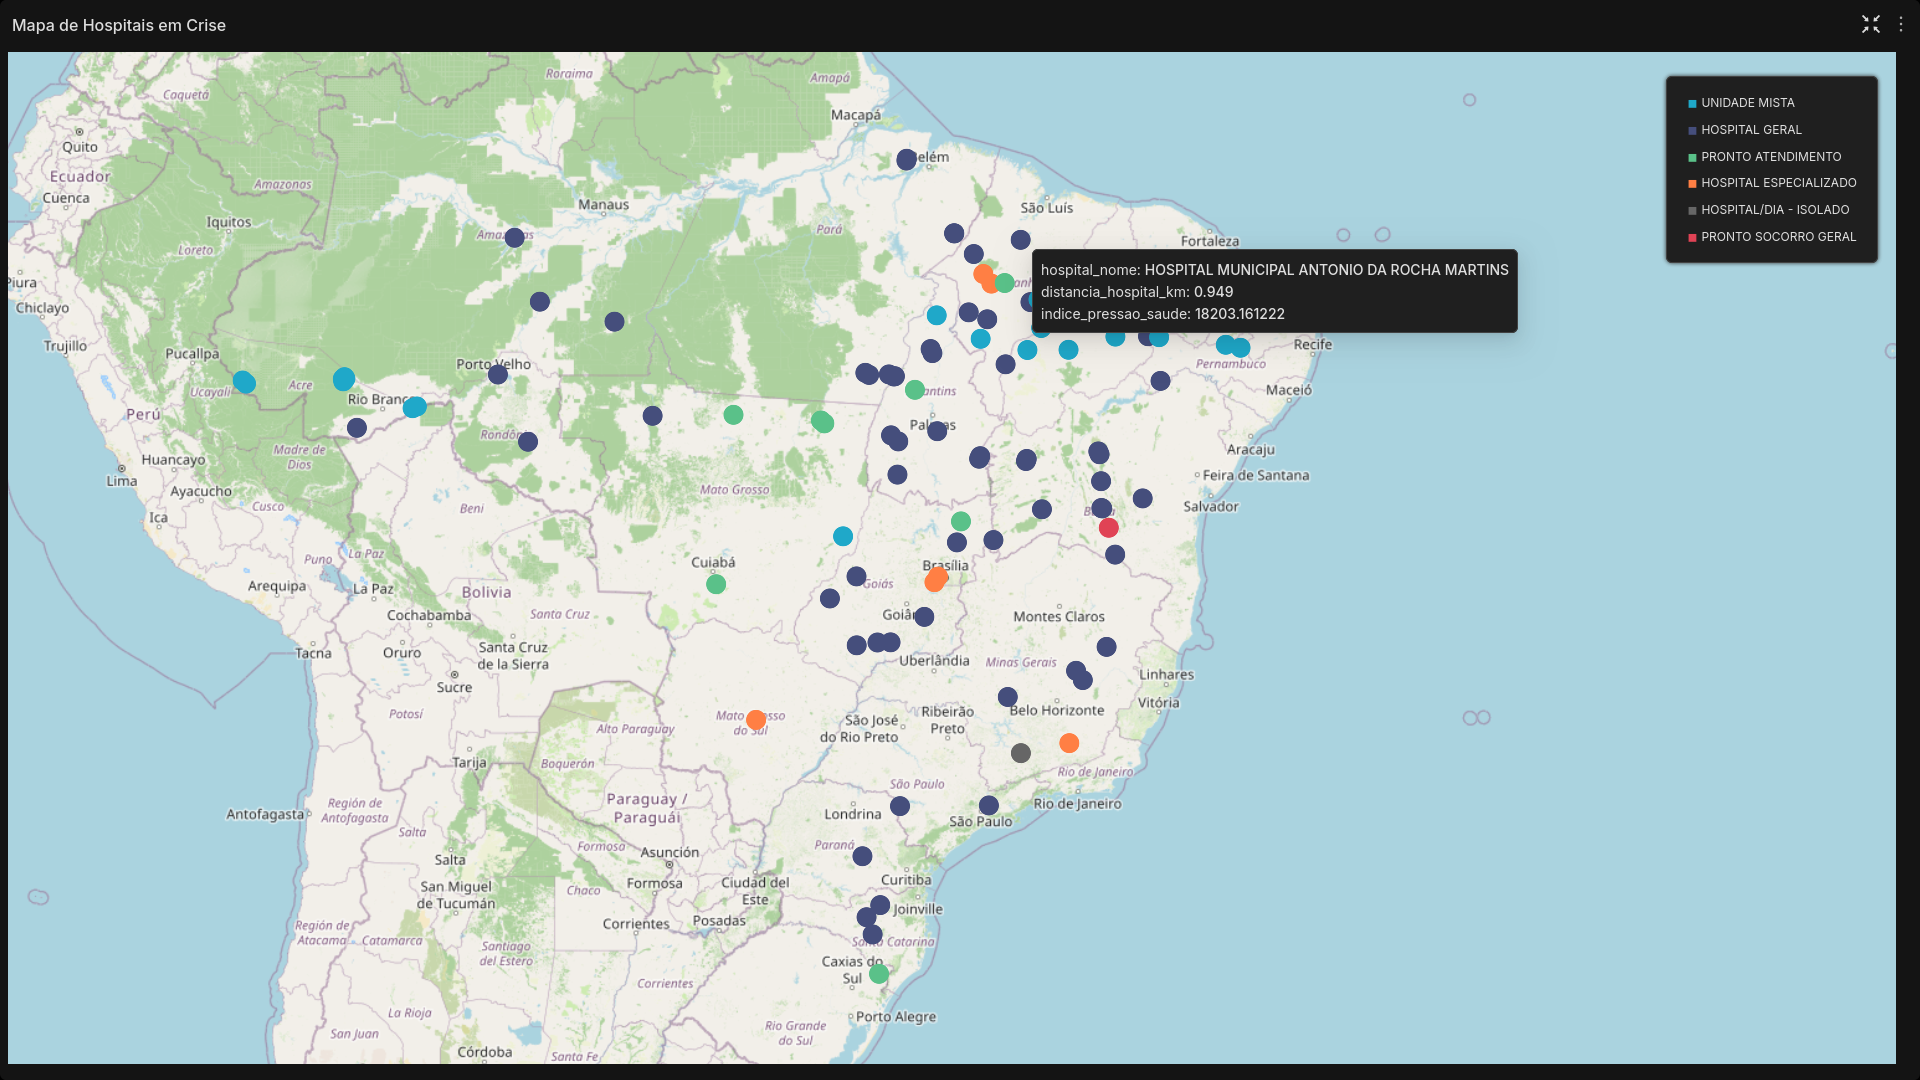
\includegraphics[width=0.9\textwidth]{materiais_apoio/figures/HospitaisCriticos.png}
    \caption{Monitoramento de Hospitais Expostos ao Fogo.}
    \label{fig:hospitais_criticos}
\end{figure}

Da mesma forma sistêmica, os dados estenderam o cordão sanitário para resguardar a malha operada pelo Operador Nacional do Sistema Elétrico (ONS). A exposição das linhas de transmissão a focos de calor intenso gera o perigo extremo de arcos elétricos e curtos-circuitos da rede neutra para a terra (desligamento forçado). 

A Figura \ref{fig:evolucao_energia} modela a progressão sistêmica dessa ameaça ao longo de todo o ano de 2025. A série temporal atua como uma evidência analítica crucial para demonstrar a assimetria da crise: o índice permanece baixo no primeiro semestre e cresce de forma acentuada a partir de setembro e outubro nas regiões de escoamento energético. Essa métrica expõe como as condições de seca extrema submetem repentinamente a infraestrutura a um aumento de pressão crítico e de complexa mitigação logística.

\begin{figure}[H]
    \centering
    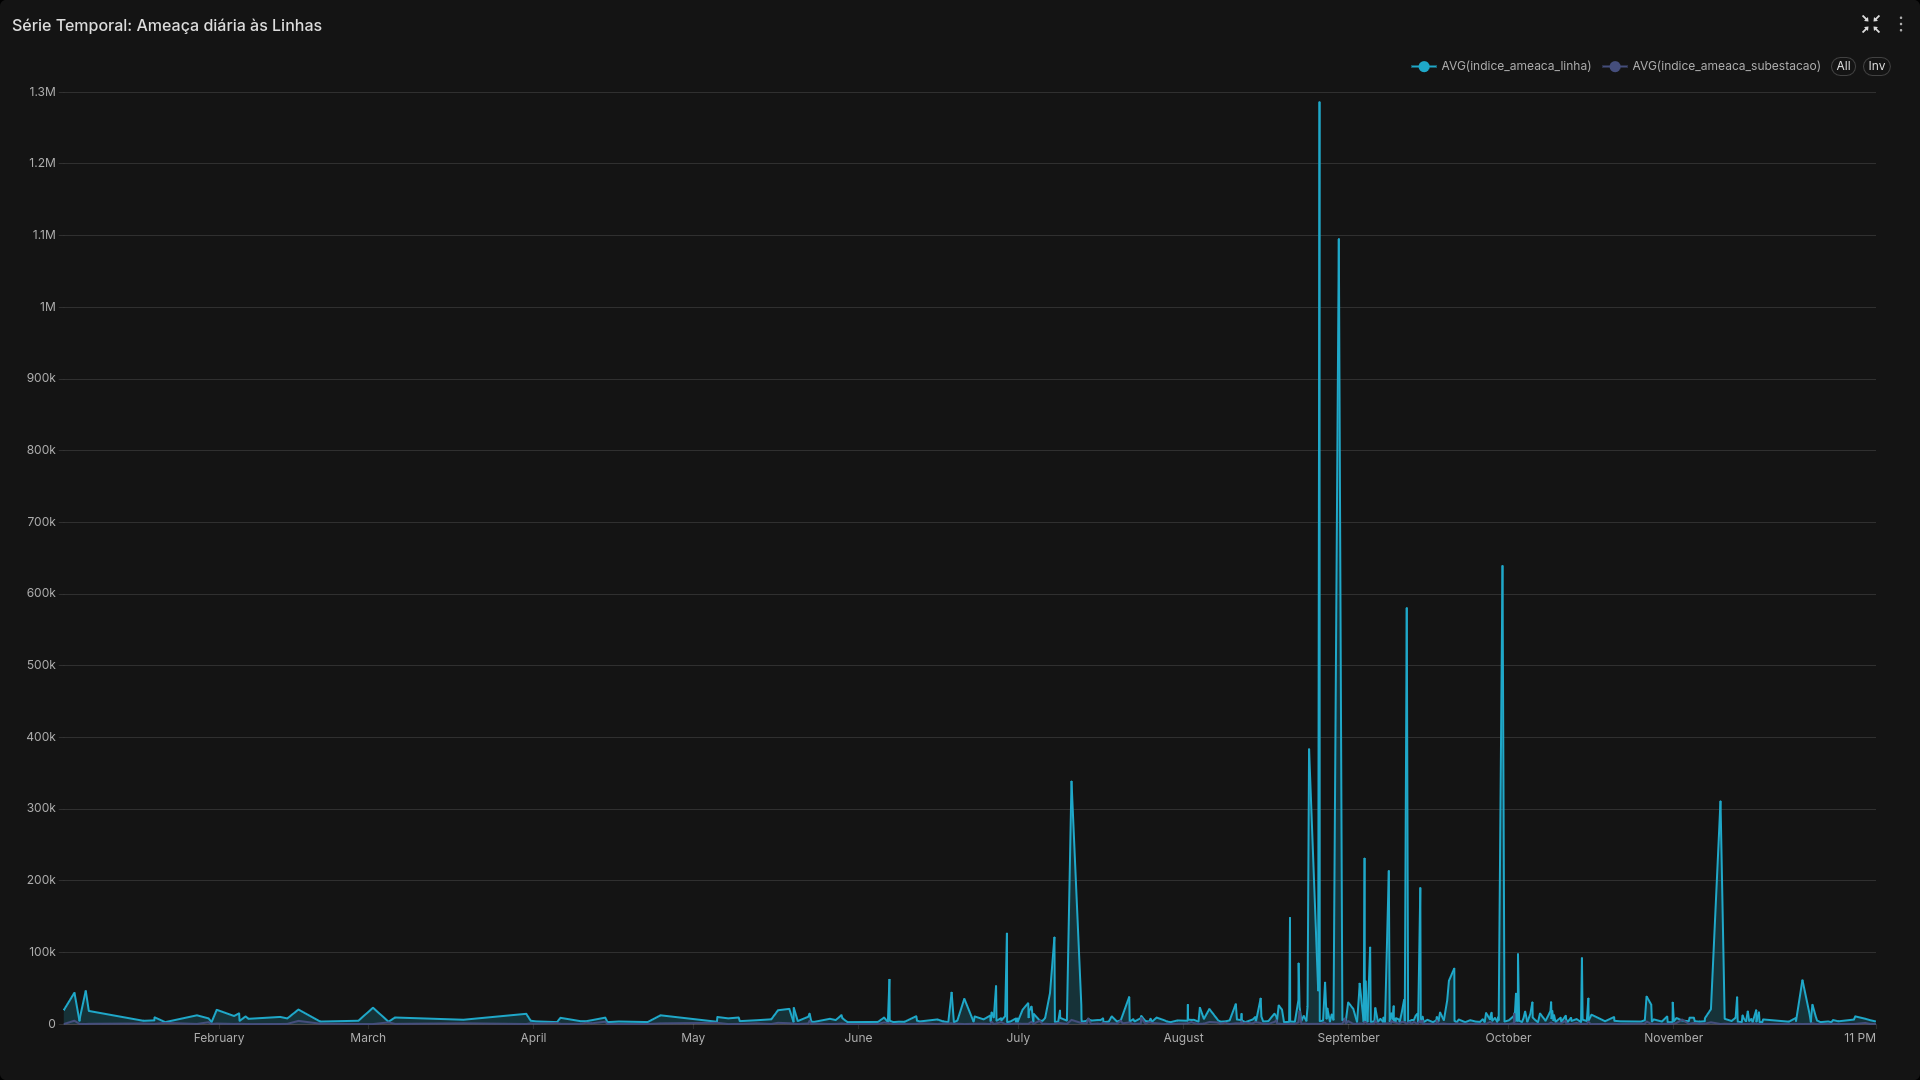
\includegraphics[width=0.9\textwidth]{materiais_apoio/figures/EvoluçãoDaPressãoEletricaAolongodoAno.png}
    \caption{Evolução da Ameaça à Infraestrutura Elétrica (ONS).}
    \label{fig:evolucao_energia}
\end{figure}

Aliando o risco termal agudo com as métricas topológicas (\textit{Betweenness Centrality}) previamente estabelecidas, a plataforma consolidou a Tabela \ref{tab:subestacoes_ameacadas}. Ela enumera as subestações mais expostas a interrupções operacionais, ordenadas pelo potencial de indução de risco sistêmico em rede. O cruzamento destacou vértices infraestruturais vitais, a exemplo da SE Rio Verde Norte (GO), elo de escoamento do Norte para o Sudeste; da SE Assis (SP), coletora da bacia do Rio Paraná; e da SE Trindade (GO), pivô na interligação Norte-Sul \cite{epe_pde_2032, ons_mapa_2026}.

Quando nós de energia sob Risco \textbf{Extremo} sofrem desligamento forçado, a matriz energética redistribui a carga base por rotas mais longas. Esse fenômeno sobrecarrega linhas secundárias e aciona sistemas primários de proteção (como o Esquema Regional de Alívio de Carga - ERAC), culminando no risco agudo de apagões regionais e blecautes em cascata por todo o subsistema interligado do país \cite{ons_procedimentos_2026}.

\begin{table}[H]
\centering
\caption{Top 10 Subestações Críticas via Betweenness Centrality.}
\label{tab:subestacoes_ameacadas}
\resizebox{\textwidth}{!}{%
\begin{tabular}{lrrc}
\toprule
\textbf{Subestação} & \textbf{Capacidade (MW)} & \textbf{Betweenness Centrality} & \textbf{Risco Cascata} \\
\midrule
R.VERDE NORTE & 1344.00 & 100.00 & EXTREMO \\
ASSIS & 2808.00 & 98.21 & EXTREMO \\
TRINDADE & 1600.00 & 91.33 & EXTREMO \\
SAMAMBAIA & 6000.00 & 89.30 & EXTREMO \\
XAVANTES & 600.00 & 89.22 & EXTREMO \\
BANDEIRANTES & 2542.00 & 87.68 & EXTREMO \\
LONDRINA ESU & 2016.00 & 59.42 & ALTO \\
BOM.JES.LAPA II & 850.00 & 47.07 & MEDIO \\
LUZIANIA & 450.00 & 46.83 & MEDIO \\
MIRACEMA & 10359.00 & 45.51 & MEDIO \\
\bottomrule
\end{tabular}%
}
\end{table}



\section{Conclusões}

Esta pesquisa aplicou o paradigma \textit{DataOps} para construir uma plataforma analítica de Defesa Civil, mitigando a fragmentação de bases institucionais (INPE, FUNAI, ANEEL, DATASUS, DNIT e IBGE). A análise do cenário evidenciou forte sazonalidade das anomalias térmicas a partir de setembro, impulsionada por secas prolongadas. O cruzamento espacial demonstrou que o avanço das chamas transcendeu a degradação florestal, exercendo pressão aguda sobre territórios indígenas e infraestruturas críticas civis, com destaque para a vulnerabilidade da malha de transmissão de energia frente ao calor convectivo e a exposição de hospitais às massas de fumaça.

Sob a ótica metodológica, o estudo atestou o valor da unificação entre ciência de redes e geoprocessamento. A formulação de um Índice de Pressão, atrelando a intensidade radiativa dos satélites (FRP) à vulnerabilidade civil, permitiu classificar as ameaças com maior embasamento quantitativo. Complementarmente, a aplicação da teoria dos grafos através da biblioteca \textit{NetworkX} viabilizou a modelagem do Risco Sistêmico, fornecendo uma base lógica para identificar os vértices estruturais da rede elétrica cuja falha poderia induzir apagões em cascata.

Tecnicamente, os resultados indicam a viabilidade do ecossistema proposto, erigido integralmente sobre ferramentas de código aberto (\textit{open-source}). A orquestração declarativa (Dagster) e os fluxos desacoplados (Apache Kafka) compuseram a infraestrutura base do sistema. No \textit{front} analítico, testado empiricamente, o Esquema Constelação no Apache Druid demonstrou capacidade para indexar grandes volumes de anomalias térmicas, sustentando agregações de baixa latência e filtragens espaciais, mesmo sob limites estritos de processamento.

Por fim, conclui-se que o arcabouço tecnológico estruturado atua como um facilitador técnico para os órgãos de resposta a emergências. A pesquisa indica que a latência e o isolamento na correlação de dados geoespaciais em larga escala podem ser consideravelmente minimizados através de uma arquitetura \textit{DataOps} integrada. Dessa forma, espera-se que o sistema contribua como uma ferramenta analítica de apoio, fornecendo insumos estruturados para embasar a tomada de decisão frente à crescente complexidade dos desastres ambientais.

\section*{Agradecimentos}

Os autores agradecem ao Conselho Nacional de Desenvolvimento Científico e Tecnológico (CNPq) e à Universidade Federal de Itajubá (UNIFEI) pelo apoio acadêmico, financeiro e de infraestrutura fundamentais para a realização desta pesquisa.

\vspace{3.5cm}

\begin{center}
    \begin{minipage}[t]{0.45\textwidth}
        \centering
        \rule{\linewidth}{0.5pt}\\
        Gabriel Gonçalves Sampaio\\
        Bolsista de Iniciação Científica (IC)
    \end{minipage}
    \hfill
    \begin{minipage}[t]{0.45\textwidth}
        \centering
        \rule{\linewidth}{0.5pt}\\
        Profª. Dra. Barbara Pimenta Caetano\\
        Professora Orientadora (PQ)
    \end{minipage}
\end{center}


\newpage
\bibliographystyle{plain}
\bibliography{referencias}

\end{document}
